%************************************************
\chapter{Decoding Movement-Related Brain Activity}\label{movement-related}
%**************************************
\begin{startbox}{ConvNets can perform as well as FBCSP on movement-related decoding}
\item Shallow network performs best on highpassed data
\item Deep network strongly benefits from cropped training on non-highpassed data
\item Residual network performs well with right initialization
\item Methodological improvements from computer vision improve EEG deep learning decoding
\item Visualizations reveal use of spectral power features with neurophysiologically plausible patterns
\end{startbox}

    Movement-related decoding problems are among the most researched in EEG
decoding and were hence our problem of choice for the first evaluation
of deep learning on EEG. A typical movement-related experimental setting
is that subjects receive a cue for a specific body part (e.g.~right
hand, feet, tongue, etc.) and either move (motor execution) or imagine
to move (motor imagery) this body part. The EEG signals recorded during
the imagined or executed movements often contain patterns specific
to the body part being moved or thought about. These patterns can then
be decoded using machine learning. In the following, I will describe our
study on movement-related EEG decoding using deep learning, mostly using
content adapted from \citet{schirrmeisterdeephbm2017} and
from \citep{hartmann2018hierarchical}. 

The main study as published in \citet{schirrmeisterdeephbm2017} was carried out
by me as the main author with help of al the coauthors. For
\citet{hartmann2018hierarchical}, Kay Hartmann was the main
contributor and I supported and advised him.

\section{Datasets}\label{datasets}

\subsection{High-Gamma Dataset}\label{high-gamma-dataset}

    Our High-Gamma Dataset is a 128-electrode dataset (of which we later
only use 44 sensors covering the motor cortex) obtained from 14 healthy
subjects (6 female, 2 left-handed, age
27.2$\pm$3.6 (mean$\pm$std)) with roughly 1000 (963.1$\pm$150.9, mean$\pm$std)
four-second trials of executed movements divided into 13 runs per
subject. The four classes of movements were movements of either the left
hand, the right hand, both feet, and rest (no movement, but same type of
visual cue as for the other classes). The training set consists of the
approx. 880 trials of all runs except the last two runs, the test set of
the approx. 160 trials of the last 2 runs. This dataset was acquired in
an EEG lab optimized for non-invasive detection of high-frequency
movement-related EEG components
\citep{ball_movement_2008,darvas_high_2010}. Such
high-frequency components in the range of approx. 60 to above 100 Hz are
typically increased during movement execution and may contain useful
movement-related information
\citep{crone_functional_1998,hammer_predominance_2016,quandt_single_2012}.
Our technical EEG Setup comprised (1.) Active electromagnetic shielding:
optimized for frequencies from DC --- 10 kHz (-30 dB to -50 dB), shielded
window, ventilation \& cable feedthrough (mrShield, CFW EMV-Consulting
AG, Reute, CH) (2.) Suitable amplifiers: high-resolution (24
bits/sample) and low-noise (\textless{}0.6 $\mu V$ RMS 0.16--200 Hz,
1.5 $\mu V$ RMS 0.16--3500 Hz), 5 kHz sampling rate (NeurOne, Mega
Electronics Ltd, Kuopio, FI) (3.) actively shielded EEG caps: 128
channels (WaveGuard Original, ANT, Enschede, NL) and (4.) full optical
decoupling: All devices are battery powered and communicate via optic
fibers.

Subjects sat in a comfortable armchair in the dimly lit Faraday cabin.
The contact impedance from electrodes to skin was typically reduced
below 5 kOhm using electrolyte gel (SUPER-VISC, EASYCAP GmbH,
Herrsching, GER) and blunt cannulas. Visual cues were presented using a
monitor outside the cabin, visible through the shielded window. The
distance between the display and the subjects' eyes was approx. 1 m. A
fixation point was attached at the center of the screen. The subjects
were instructed to relax, fixate the fixation mark and to keep as still
as possible during the motor execution task. Blinking and swallowing was
restricted to the inter-trial intervals. The electromagnetic shielding
combined with the comfortable armchair, dimly lit Faraday cabin and the
relatively long 3-4 second inter-trial intervals (see below) were used
to minimize artifacts produced by the subjects during the trials.

The tasks were as following. Depending on the direction of a gray arrow
that was shown on black background, the subjects had to repetitively
clench their toes (downward arrow), perform sequential finger-tapping of
their left (leftward arrow) or right (rightward arrow) hand, or relax
(upward arrow). The movements were selected to require little proximal
muscular activity while still being complex enough to keep subjects
involved. Within the 4-s trials, the subjects performed the repetitive
movements at their own pace, which had to be maintained as long as the
arrow was showing. Per run, 80 arrows were displayed for 4 s each, with
3 to 4 s of continuous random inter-trial interval. The order of
presentation was pseudo-randomized, with all four arrows being shown
every four trials. Ideally 13 runs were performed to collect 260 trials
of each movement and rest. The stimuli were presented and the data
recorded with BCI2000 \citep{schalk_bci2000:_2004}. The
experiment was approved by the ethical committee of the University of
Freiburg.

\subsection{BCI Competition IV 2a}\label{bci-competition-iv-2a}

    The BCI competition IV dataset 2a is a 22-electrode EEG motor-imagery
dataset, with 9 subjects and 2 sessions, each with 288 four-second
trials of imagined movements per subject (movements of the left hand,
the right hand, the feet and the tongue), for details see
\citet{brunner_bci_2008}. The training set consists of the
288 trials of the first session, the test set of the 288 trials of the
second session.

\subsection{BCI Competition IV 2b}\label{bci-competition-iv-2b}

    The BCI competition IV dataset 2b is a 3-electrode EEG motor-imagery
dataset with 9 subjects and 5 sessions of imagined movements of the left
or the right hand, the latest 3 sessions include online feedback
\citep{leeb_bci_2008}. The training set consists of the
approx. 400 trials of the first 3 sessions
(408.9$\pm$13.7, mean$\pm$std), the test set consists of the approx. 320 trials (315.6$\pm$12.6, mean$\pm$std)of the last two sessions.

\section{Preprocessing}

    We only minimally preprocessed the data to allow the networks to extract
as much information as possible while keeping the input distribution in
a value range suitable for stable network training.

Concretely, our preprocessing steps were:

\begin{enumerate}
\item
  \textbf{Remove outlier trials:} Any trial where at least one channel
  had a value outside +- 800 mV was removed to ensure stable training.
\item
  \textbf{Channel selection:} For the high-gamma dataset, we selected
  only the 44 sensors covering the motor cortex for faster and more
  accurate motor decoding.
\item
  \textbf{High/Bandpass (optional) :} Highpass signal to above 4 Hz.
  This should partially remove potentially informative eye components
  from the signal and ensure that the decoding relies more on brain
  signals. For the BCI competition datasets, in this step we bandpassed
  to 4-38 Hz as using only frequencies until \textasciitilde38-40 Hz was
  commonly done in prior work in this dataset.
\item
  \textbf{Standardization:} Exponential moving standardization as
  described below to make sure the input distribution value range is
  suitable for network training.
\end{enumerate}

Our electrode-wise exponential moving standardization computes
exponential moving means and variances with a decay factor of 0.999 for
each channel and used these to standardize the continuous data.
Formally,

\begin{align}
\mu_t &= 0.001 x_t + 0.999\mu_{t-1}\\
\sigma_t^2 &= 0.001(x_t - \mu_t)^2 + 0.999 \sigma_{t-1}^2\\
x't &= (x_t - \mu_t) / \sqrt{\sigma_t^2}\\
\end{align}

where $x't$ and $x_t$ are the standardized and the original signal
for one electrode at time $t$, respectively. As starting values for
these recursive formulas we set the first 1000 mean values $\mu_t$ and
first 1000 variance values $\sigma_t^2$ to the mean and the variance
of the first 1000 samples, which were always completely inside the
training set (so we never used future test data in our preprocessing).
Some form of standardization is a commonly used procedure for ConvNets;
exponentially moving standardization has the advantage that it is also
applicable for an online BCI.

For FBCSP, this standardization always worsened accuracies in
preliminary experiments, so we did not use it. Overall, the minimal
preprocessing without any manual feature extraction ensured our
end-to-end pipeline could in principle be applied to a large number of
brain-signal decoding tasks as we validated later, see
\Cref{task-related}.

\section{Training Details}\label{training-details}

    As our optimization method, we used Adam
\cite{kingma_adam:_2014} together with a specific early
stopping method, as this consistently yielded good accuracy in
preliminary experiments on the training set. Adam is a variant of
stochastic gradient descent designed to work well with high-dimensional
parameters, which makes it suitable for optimizing the large number of
parameters of a ConvNet \cite{kingma_adam:_2014}. The early
stopping strategy that we use throughout these experiments, developed in
the computer vision field \footnote{https://web.archive.org/web/20160809230156/https://code.google.com/p/cuda-convnet/wiki/Methodology},
splits the training set into a training and validation fold and stops
the first phase of the training when validation accuracy does not
improve for a predefined number of epochs. The training continues on the
combined training and validation fold starting from the parameter values
that led to the best accuracies on the validation fold so far. The
training ends when the loss function on the validation fold drops to the
same value as the loss function on the training fold at the end of the
first training phase (we do not continue training in a third phase as in
the original description). Early stopping in general allows training on
different types of networks and datasets without choosing the number of
training epochs by hand. Our specific strategy uses the entire training
data while only training once. In our study, all reported accuracies
have been determined on an independent test set.

    Note that in later works we do not use this early stopping method
anymore as we found training on the whole training set with a cosine
learning rate schedule \cite{DBLP:conf/iclr/LoshchilovH17} to
lead to better final decoding performance.

\section{Design Choices}\label{design-choices}



\begin{table}[ht]
    \small
    \myfloatalign
    \begin{tabularx}{\textwidth}{p{0.16\textwidth}p{0.16\textwidth}p{0.16\textwidth}p{0.4\textwidth}} \toprule
        \tableheadlinewithwidth{0.16\textwidth}{\large Design aspect} &
        \tableheadlinewithwidth{0.16\textwidth}{\large Our Choice} & \tableheadlinewithwidth{0.16\textwidth}{\large Variants} & \tableheadlinewithwidth{0.4\textwidth}{\large Motivation}\\ 
        \midrule
    Activation functions & ELU & Square, ReLU & We expected these choices to
be sensitive to the type of feature (e.g., signal phase or power), as
squaring and mean pooling results in mean power (given a zero-mean
signal). Different features may play different roles in the
low-frequency components vs the higher frequencies (see the section
``Datasets and Preprocessing''). \\
Pooling mode & Max & Mean & (see above) \\
Regulariza-tion and intermediate normalization & Dropout + batch normalization + a new tied loss function (explanations see text) &Only
 batch normalization, only dropout, neither of both, nor tied loss & We
wanted to investigate whether recent deep learning advances improve
accuracies and check how much regularization is required. \\
Factorized temporal convolutions & One 10 x 1 convolution per
convolutional layer & Two 6 x 1 convolutions per convolutional layer &
Factorized convolutions are used by other successful ConvNets \citep{szegedy_rethinking_2015} \\
Splitted vs one-step convolution & Splitted convolution in first layer (see \Cref{shallow-convnet-architecture}) &  One-step
convolution in first layer & Factorizing convolution into spatial and
temporal parts may improve accuracies for the large number of EEG input
channels (compared with three rgb color channels of regular image
datasets). \\
        \bottomrule
    \end{tabularx}
    \caption[Evaluated design choices]{\textbf{Evaluated design choices.}}  
    \label{design-choices-table}
\end{table}


For the shallow and deep network, we evaluated how a number of design
choices affect the final accuracies, see \Cref{design-choices-table}.

\subsection{Tied Loss Function}\label{tied-loss-function}

Our tied loss function penalizes the discrepancy between neighbouring
predictions. Concretely, in this \emph{tied sample loss function}, we
added the cross-entropy of two neighboring predictions to the usual loss
of of negative log likelihood of the labels. So, denoting the predicted
probabilties $p\big(l_k|f_k(X^j_{t..t+T'};\theta)\big)$ for crop
$X^j_{t..t+T'}$ with label $l_k$ from time step $t$ to $t+T'$ by
$p_{f,k}(X^j_{t..t+T'})$, the loss now also depends on the predicted
probabilties for the next crop $p_{f,k}(X^j_{t..t+T'+1})$ and is then:
% 

\begin{equation}
\begin{split}
 \textrm{loss}\big(y^j, p_{f,k}(X^j_{t..t+T'})\big) &= \sum_{k=1}^{K}-log\big(p_{f,k}(X^j_{t..t+T'})\big)\cdot \delta(y^j=l_k) \\
 &+ \sum_{k=1}^{K}-log\big(p_{f,k}(X^j_{t..t+T'})\big) \cdot p_{f,k}(X^j_{t..t+T'+1})
\end{split}
\end{equation}



This is meant to make the ConvNet focus on features which are stable for
several neighboring input crops.

\section{Results}\label{results}

\subsection{Validation of FBCSP Pipeline}\label{validation-of-fbcsp-pipeline}

    As a first step before moving to the evaluation of ConvNet decoding, we
validated our FBCSP implementation, as this was the baseline we compared
the ConvNets results against. To validate our FBCSP implementation, we
compared its accuracies to those published in the literature for the BCI
competition IV dataset 2a \citep{sakhavi_parallel_2015}.
Using the same 0.5--2.5 s (relative to trial onset) time window, we
reached an accuracy of 67.6\%, statistically not significantly different
from theirs (67.0\%, p=0.73, Wilcoxon signed-rank test). Note however,
that we used the full trial window for later experiments comparing
against convolutional networks, i.e., from 0.5--4 seconds. This yielded
a slightly better accuracy of 67.8\%, which was still not statistically
significantly different from the original results on the 0.5--2.5 s
window (p=0.73). For all later comparisons, we use the 0.5--4 seconds
time window on all datasets.

\subsection{Filterbank Network}\label{filterbank-network}

\begin{table}[ht]
    \myfloatalign
    \begin{tabularx}{\textwidth}{llll}
    \toprule
        \tableheadlinewithwidth{0.2\textwidth}{Decoding method} & \tableheadlinewithwidth{0.2\textwidth}{Sampling rate} &
        \tableheadlinewithwidth{0.2\textwidth}{Test Accuracy [\%]}  & 
        \tableheadlinewithwidth{0.2\textwidth}{Std [\%]} 
        \\
        \midrule
        FBCSP & 300 & 88.1 & 13.9 \\
        FBCSP & 150 & 86.7 & 14.3 \\
        Filterbank Net & 300 & 90.5 & 10.4 \\
        Filterbank Net & 150 & 87.9 & 13.9 \\
        \bottomrule
    \end{tabularx}
    \caption[Filterbank Net vs FBCSP Accuracies.]{\textbf{Filterbank Net vs FBCSP Accuracies.} Std is standard deviation over the 18 subjects used here. Results from \citet{schirrmeister_msc_thesis_2015}.}  \label{filterbank-net-results}
\end{table}


    Prior to our more extensive study, we had evaluated the filterbank
network on a different version of the High-Gamma Dataset in a master
thesis \citep{schirrmeister_msc_thesis_2015}. This version
of the dataset included different subjects, as some subjects had not
been recorded yet and other subjects were later excluded for the work
here due to the presence of too many artifacts. Furthermore, we
evaluated 150Hz and 300 Hz as sampling rates here, in the remainder we
will use 250 Hz.

The results in \Cref{filterbank-net-results} show that the
Filterbank net outperformed FBCSP by 2.4\% (300 Hz) and 1.3\% (150 Hz)
respectively. Despite the good performance, we did not evaluate this
network further after the master thesis due to the very large GPU memory
requirement of our implementation and our interest in evaluating more
expressive architectures not as tightly constrained to implement FBCSP
steps.

\subsection{ConvNets Reached FBCSP
Accuracies}\label{convnets-reached-fbcsp-accuracies}


\begin{figure}[h!tb]
    \myfloatalign
    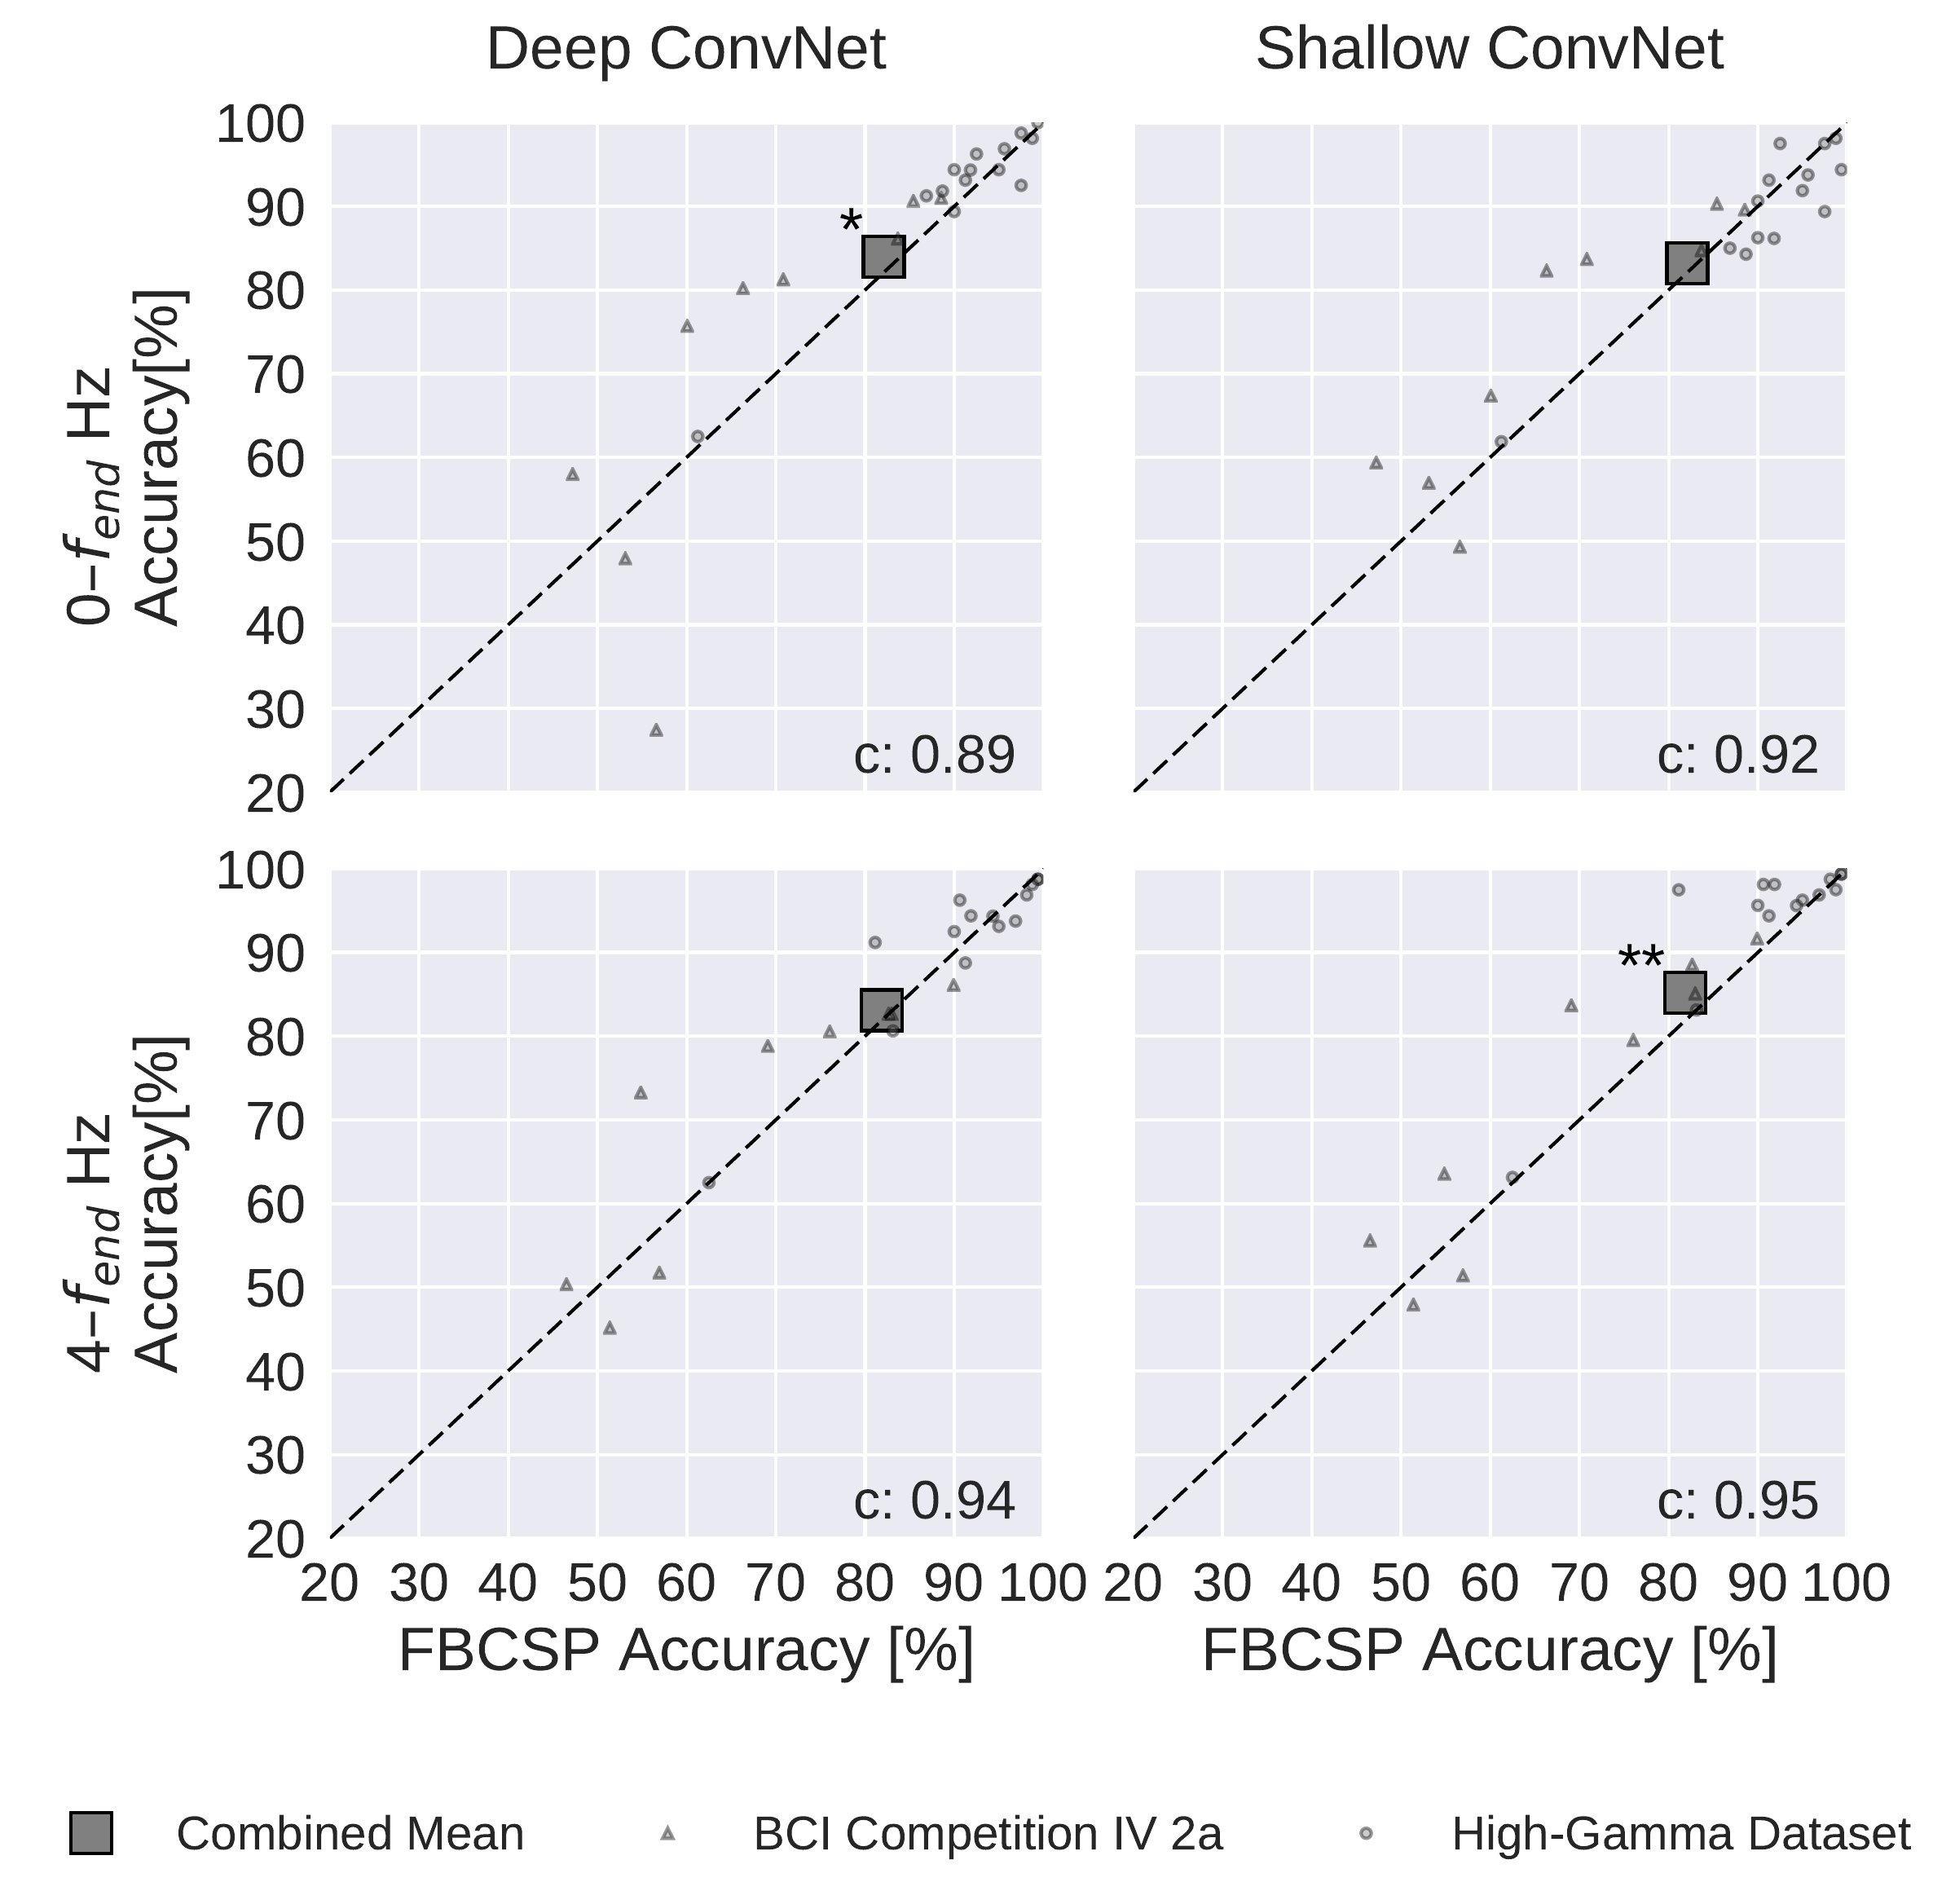
\includegraphics[width=0.9\linewidth]{images/Final_Comparison.ipynb.2.png}
    \caption[FBCSP vs. ConvNet decoding accuracies.]{
\textbf{FBCSP vs. ConvNet decoding accuracies.} Each small marker
represents accuracy of one subject, the large square markers represent
average accuracies across all subjects of both datasets. Markers above
the dashed line indicate experiments where ConvNets performed better
than FBCSP and opposite for markers below the dashed line. Stars
indicate statistically significant differences between FBCSP and
ConvNets (Wilcoxon signed-rank test, p\textless0.05: *, p\textless0.01:
**, p\textless0.001:***). Bottom left of every plot: linear correlation
coefficient between FBCSP and ConvNet decoding accuracies. Mean
accuracies were very similar for ConvNets and FBCSP, the (small)
statistically significant differences were in direction of the ConvNets.
Figure from \citet{schirrmeisterdeephbm2017}.
}
\label{movement-decoding-result-comparison-figure}
\end{figure}


\begin{table}[htb]
    \myfloatalign
    \begin{tabularx}{\textwidth}{lllll}
    \toprule
        \tableheadlinewithwidth{0.25\textwidth}{Dataset} & \tableheadlinewithwidth{0.2\textwidth}{Frequency Range (Hz)} &
        \tableheadlinewithwidth{0.12\textwidth}{FBCSP}  & 
        \tableheadlinewithwidth{0.12\textwidth}{Deep} & 
        \tableheadlinewithwidth{0.12\textwidth}{Shallow} 
        \\
        \midrule
        BCIC IV 2a & 0--38 & 68.0 & +2.9 & +5.7* \\
        BCIC IV 2a & 4--38 & 67.8 & +2.3 & +4.1 \\
        HGD & 0--125 & 91.2 & +1.3 & -1.9 \\
        HGD & 4--125 & 90.9 & +0.5 & +3.0* \\
        Combined & 0--$f_{end}$ & 82.1 & +1.9* & +1.1 \\
        Combined & 4--$f_{end}$ & 81.9 & +1.2 & +3.4** \\
        \bottomrule
    \end{tabularx}
    \caption[Deep and Shallow ConvNet vs. FBCSP Accuracies]{
    \textbf{Deep and Shallow ConvNet vs. FBCSP Accuracies.}
    FBCSP decoding accuracies and difference of deep and shallow ConvNet
    accuracies to FBCSP results are given in percentage. BCIC IV 2a: BCI
    competition IV dataset 2a. HGD: High-Gamma Dataset. Frequency range is
    in Hertz. Stars indicate statistically significant differences (P values
    from Wilcoxon signed-rank test, *: P < 0.05, **:
    P < 0.01, no P values were below 0.001). Note that all P
    values below 0.01 in this study remain significant when controlled with
    false-discovery-rate correction at $\alpha=0.05$ across all tests
    involving ConvNet accuracies.
    }  \label{deep-shallow-hgd-results}
\end{table}
 
    Both the deep and the shallow ConvNets, with appropriate design choices
(see \Cref{design-choices-results}), reached similar accuracies
as FBCSP-based decoding, with small but statistically significant
advantages for the ConvNets in some settings. For the mean of all
subjects of both datasets, accuracies of the shallow ConvNet on
$0-f_\textrm{end}$ Hz and for the deep ConvNet on $4-f_\textrm{end}$
Hz were not statistically significantly different from FBCSP (see
\Cref{movement-decoding-result-comparison-figure}). The deep
ConvNet on $0-f_\textrm{end}$ Hz and the shallow ConvNet on
$4-f_\textrm{end}$ Hz reached slightly higher (1.9\% and 3.3\% higher,
respectively) accuracies that were also statistically significantly
different (P \textless{} 0.05, Wilcoxon signed-rank test). Note that all
results in this section were obtained with cropped training. Note that
all P values below 0.01 in this study remain significant when controlled
with false-discovery-rate correction at $\alpha=0.05$ across all tests
involving ConvNet accuracies.

\section{Confusion Matrices are Similar between FBCSP and
ConvNets}\label{confusion-matrices-are-similar-between-fbcsp-and-convnets}


\begin{figure}[h!tb]
    \myfloatalign
    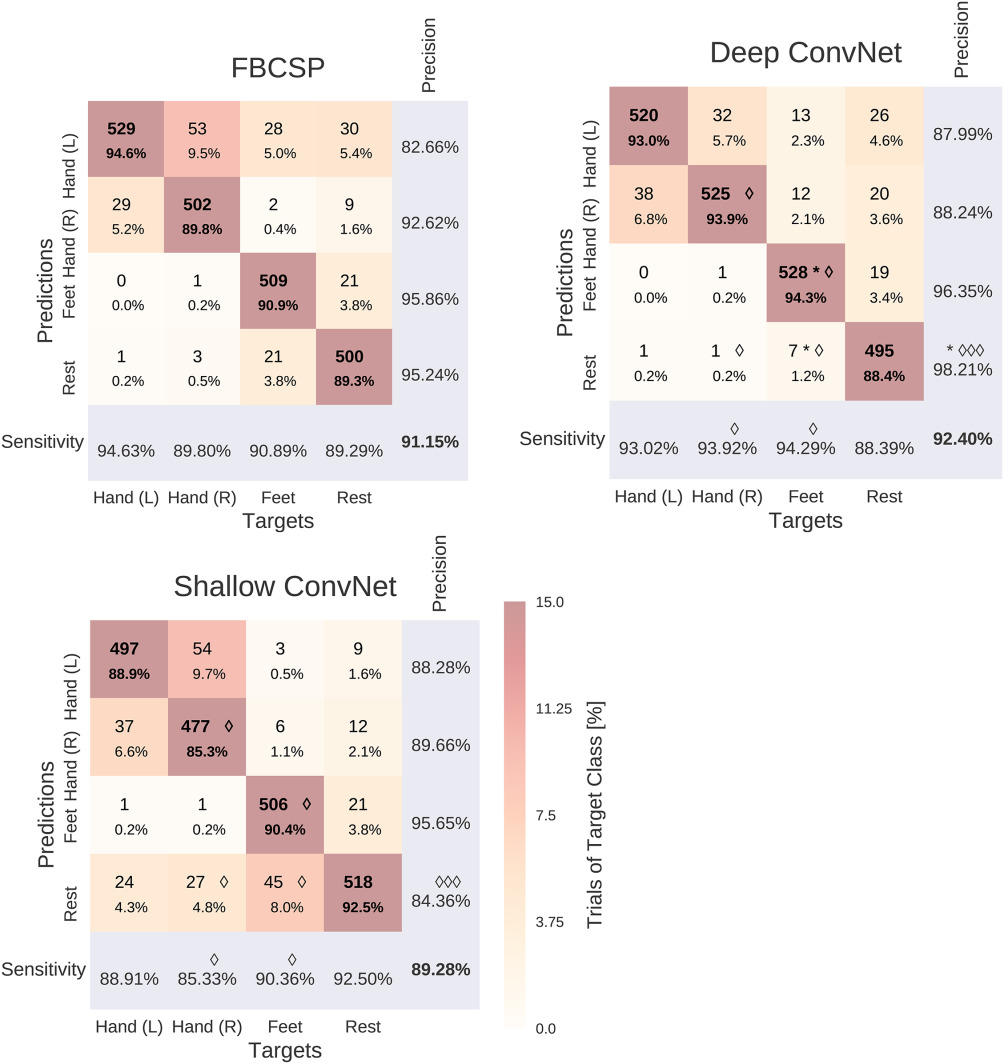
\includegraphics[width=0.9\linewidth]{images/Confusion_Mats.jpg}
    \caption[Confusion matrices for FBCSP- and ConvNet-based decoding]{
\textbf{Confusion matrices for FBCSP- and ConvNet-based decoding.}
Results are shown for the High-Gamma Dataset, on $0–f_\textrm{end}$
Hz. Each entry of row r and column c for upper-left 4×4-square: Number
of trials of target r predicted as class c (also written in percent of
all trials). Bold diagonal corresponds to correctly predicted trials of
the different classes. Percentages and colors indicate fraction of
trials of corresponding column (i.e.,
from trials of the corresponding target class). The lower-right
value corresponds to overall accuracy. Bottom row corresponds to
sensitivity
: $\frac{\mathrm{number\ of\ trials\ correctly\ predicted\ for\ 
class\ c}}{\mathrm{number\ of\ trials\ for\ class\ c}}$. Rightmost column corresponds to
precision: $\frac{\mathrm{number\ of\ trials\ correctly\ predicted\ for\ 
class\ r}}{\mathrm{number\ of\ trials\ predicted\ as\ class\ r}}$. Stars indicate statistically
significantly different values between ConvNet decoding and FBCSP, diamonds between the shallow and deep ConvNets. P\textless0.05: $\diamond$/*,
P\textless0.01: $\diamond\diamond$/**, P\textless0.001:
$\diamond\diamond\diamond$/***, Wilcoxon signed-rank test. Figure from
\citet{schirrmeisterdeephbm2017}.
}
\label{confusion-mat-figure}
\end{figure}



\begin{table}[htb]
\centering \footnotesize
\begin{tabular}{lllllll}\toprule
&
\tableheadline{\parbox{0.12\linewidth}{Hand (L)\\Hand (R)}} & 
\tableheadline{\parbox{0.12\linewidth}{Hand (L)\\Feet}} & 
\tableheadline{\parbox{0.12\linewidth}{Hand (L)\\Rest}} & 
\tableheadline{\parbox{0.12\linewidth}{Hand (R)\\Feet}} & 
\tableheadline{\parbox{0.12\linewidth}{Hand (R)\\Rest}} & 
\tableheadline{\parbox{0.05\linewidth}{Feet\\Rest}} \\\midrule
 FBCSP & 82 & 28 & 31 & 3 & 12 & 42 \\ 
 Deep & 70 & 13 & 27 & 13 & 21 & 26 \\ 
 Shallow & 99 & 3 & 34 & 5 & 37 & 73 \\ 
  \bottomrule
\hline
\end{tabular}
\caption[Decoding errors between class pairs]{\textbf{Decoding errors between class pairs.} Results for the High-Gamma Dataset.
Number of trials where one class  was mistaken for the
other for each decoding method, summed per class pair. The largest
number of errors was between Hand(L) and Hand (R) for all three
decoding methods, the second largest between Feet and Rest (on average
across the three decoding methods). Together, these two class pairs
accounted for more than 50\% of all errors for all three decoding
methods. In contrast, Hand (L and R) and Feet had a small number of
errors irrespective of the decoding method used.}
\label{hgd-class-mistakes-table} 
\end{table}

    Confusion matrices for the High-Gamma Dataset on 0--$f_{end}$ Hz were
very similar for FBCSP and both ConvNets (see
\Cref{confusion-mat-figure}). The majority of all mistakes
were due to discriminating between Hand (L) / Hand (R) and Feet / Rest,
see Table \Cref{hgd-class-mistakes-table}. Seven entries of
the confusion matrix had a statistically significant difference
(p\textless0.05, Wilcoxon signed-rank test) between the deep and the
shallow ConvNet, in all of them the deep ConvNet performed better. Only
two differences between the deep ConvNet and FBCSP were statistically
significant (p\textless0.05), none for the shallow ConvNet and FBCSP.
Confusion matrices for the BCI competition IV dataset 2a showed a larger
variability and hence a less consistent pattern, possibly because of the
much smaller number of trials.

\section{Residual ConvNets Can Be Competitive with Improved
Training}\label{residual-convnets-can-be-competitive-with-improved-training}


\begin{table}[htb]
    \myfloatalign
    \begin{tabularx}{\textwidth}{lllll}
    \toprule
        \tableheadlinewithwidth{0.25\textwidth}{Dataset} & \tableheadlinewithwidth{0.2\textwidth}{Frequency Range (Hz)} &
        \tableheadlinewithwidth{0.12\textwidth}{FBCSP}  & 
        \tableheadlinewithwidth{0.12\textwidth}{ResNet Before} & 
        \tableheadlinewithwidth{0.12\textwidth}{ResNet Now} 
        \\
        \midrule
        BCIC IV 2a & 0--38 & 68.0 & -0.3 & +3.7 \\
        BCIC IV 2a & 4--38 & 67.8 & -7.0* & -0.9 \\
        HGD & 0--125 & 91.2 & -2.3* & +1.1 \\
        HGD & 4--125 & 90.9 & -1.1 & 0.0 \\
        Combined & 0--$f_{end}$ & 82.1 & -1.1 & +2.2 \\
        Combined & 4--$f_{end}$ & 81.9 & -3.5* & -0.4 \\
        \bottomrule
    \end{tabularx}
    \caption[Residual ConvNet vs. FBCSP Accuracies]{
   \textbf{Residual ConvNet vs. FBCSP Accuracies.} Accuracies
and significance stars have same meaning as before.
    }  \label{residual-hgd-results}
\end{table}

In our original study, residual ConvNets had underperformed our FBCSP
baseline, in several settings even with statistical significance.
However, later investigations revealed that better weight
initializations, concretely scaling down the weight initialization more
strongly, can lead to improved results. In work done for this thesis, I
repeated the original experiments using our current decoding pipeline
with the residual ConvNets. \Cref{residual-hgd-results}
reports the original accuracies and the accuracies obtained with our
current codebase. Notably, residual ConvNets no longer substantially
underperform FBCSP, even slightly outperforming it in the setting
without highpass.


\section{Design Choices Affected Decoding Performance}\label{design-choices-results}



\begin{figure}[h!tb]
    \captionsetup[subfigure]{labelformat=empty}
    \myfloatalign
    \subfloat[]
    {
        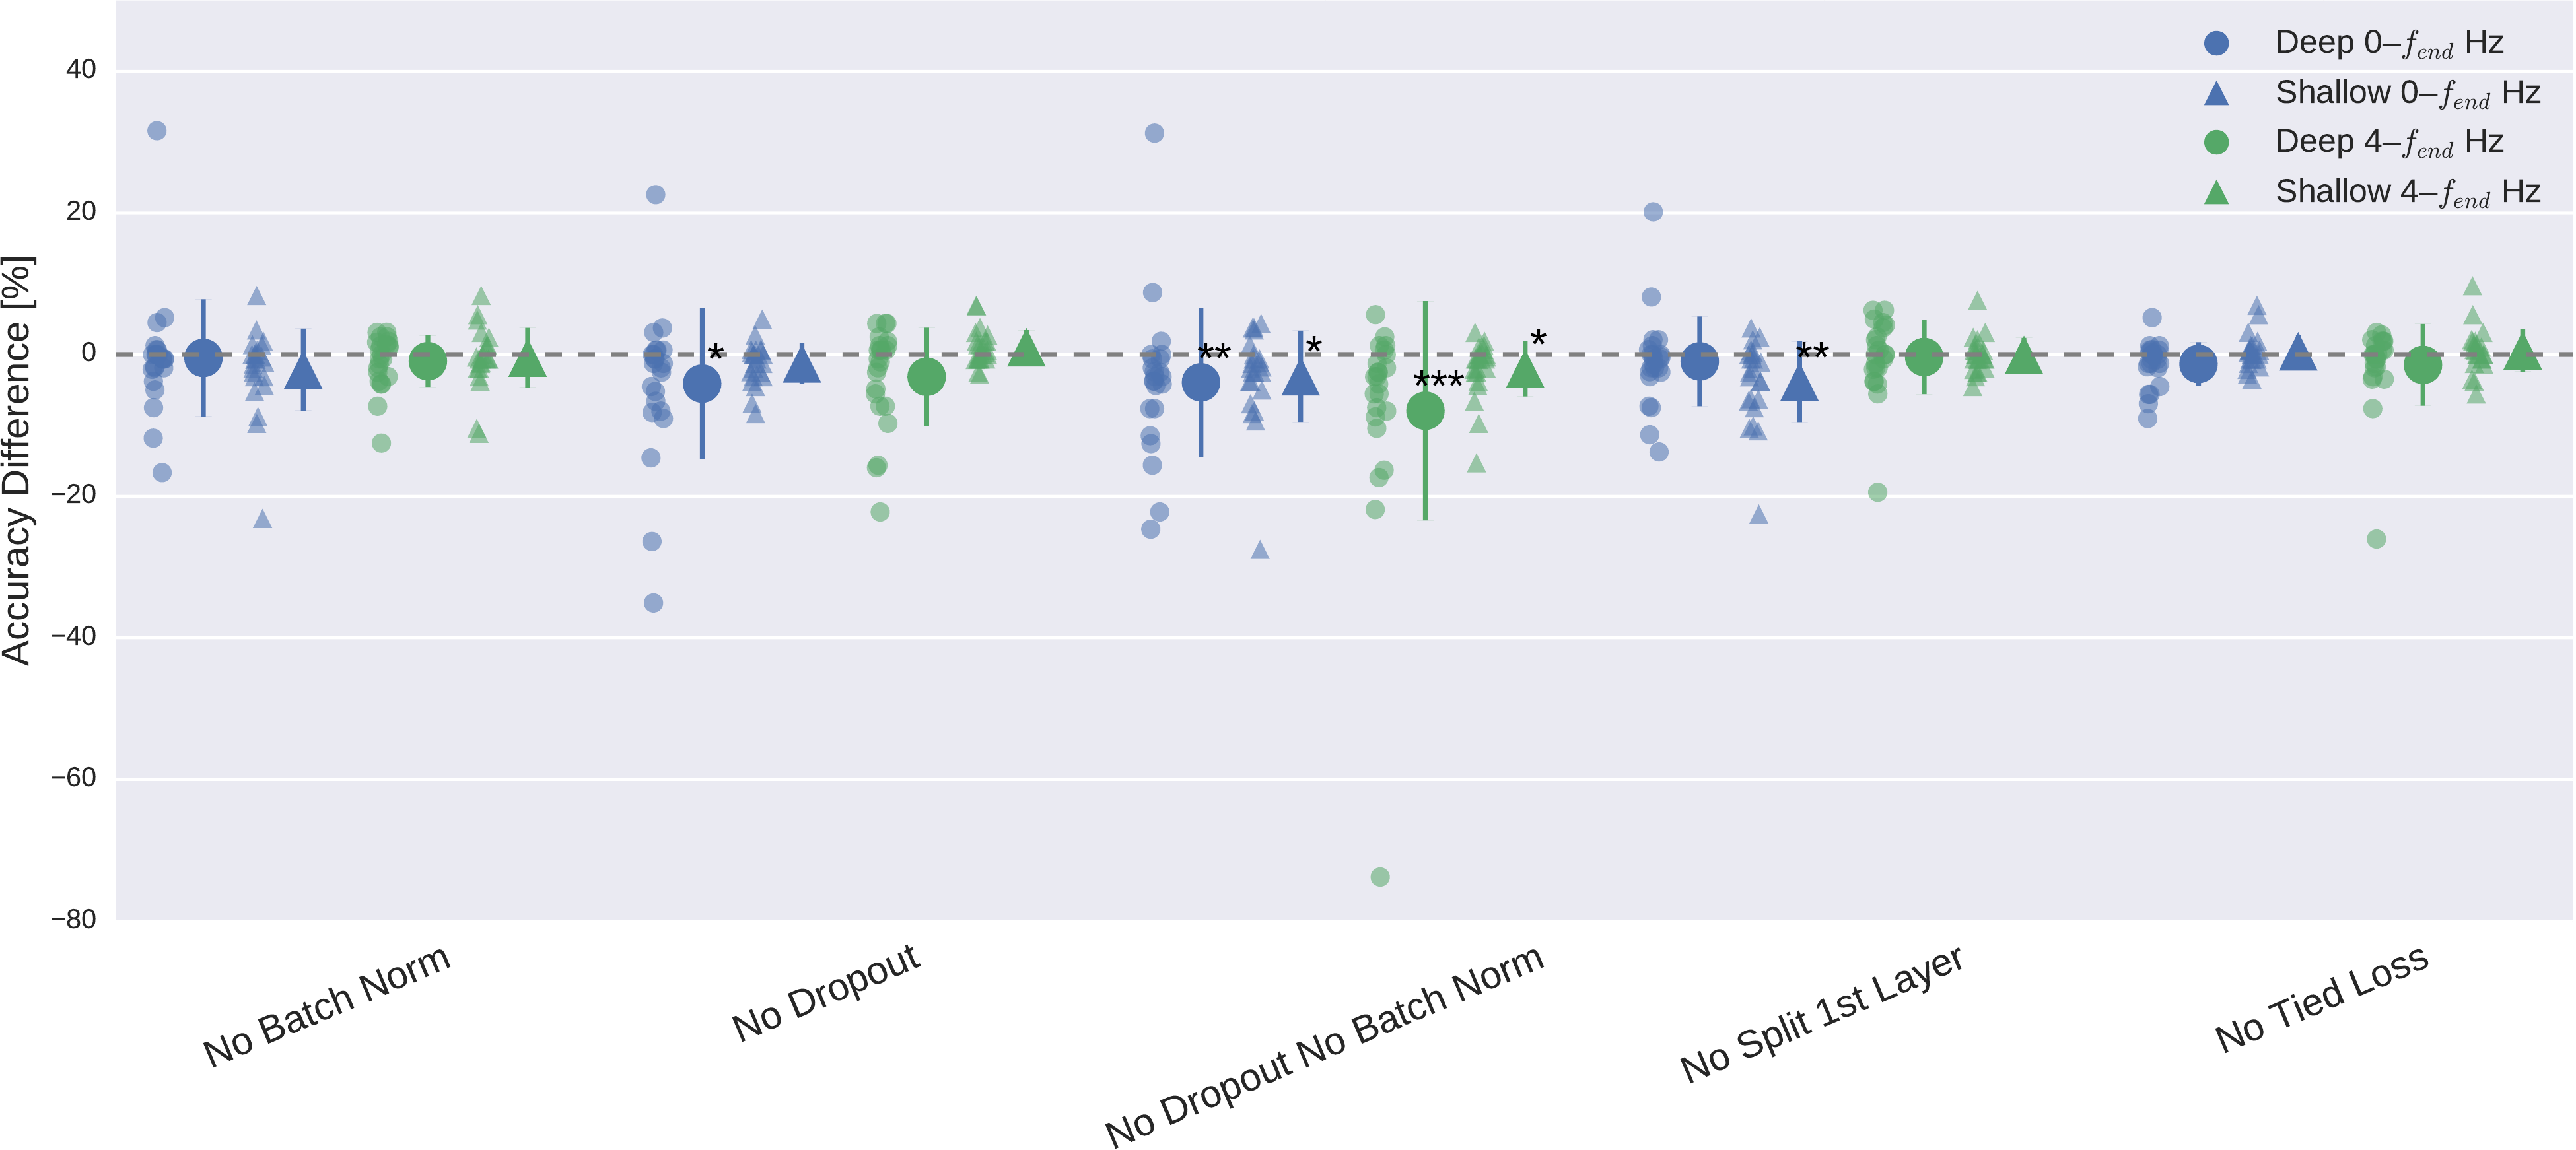
\includegraphics[width=0.9\linewidth]{images/Final_Comparison.ipynb.9.pdf-1.png} 
    } \\
    \vspace{-0.5cm}
    \subfloat[]
    {
    \label{design-choices-b-fig}
    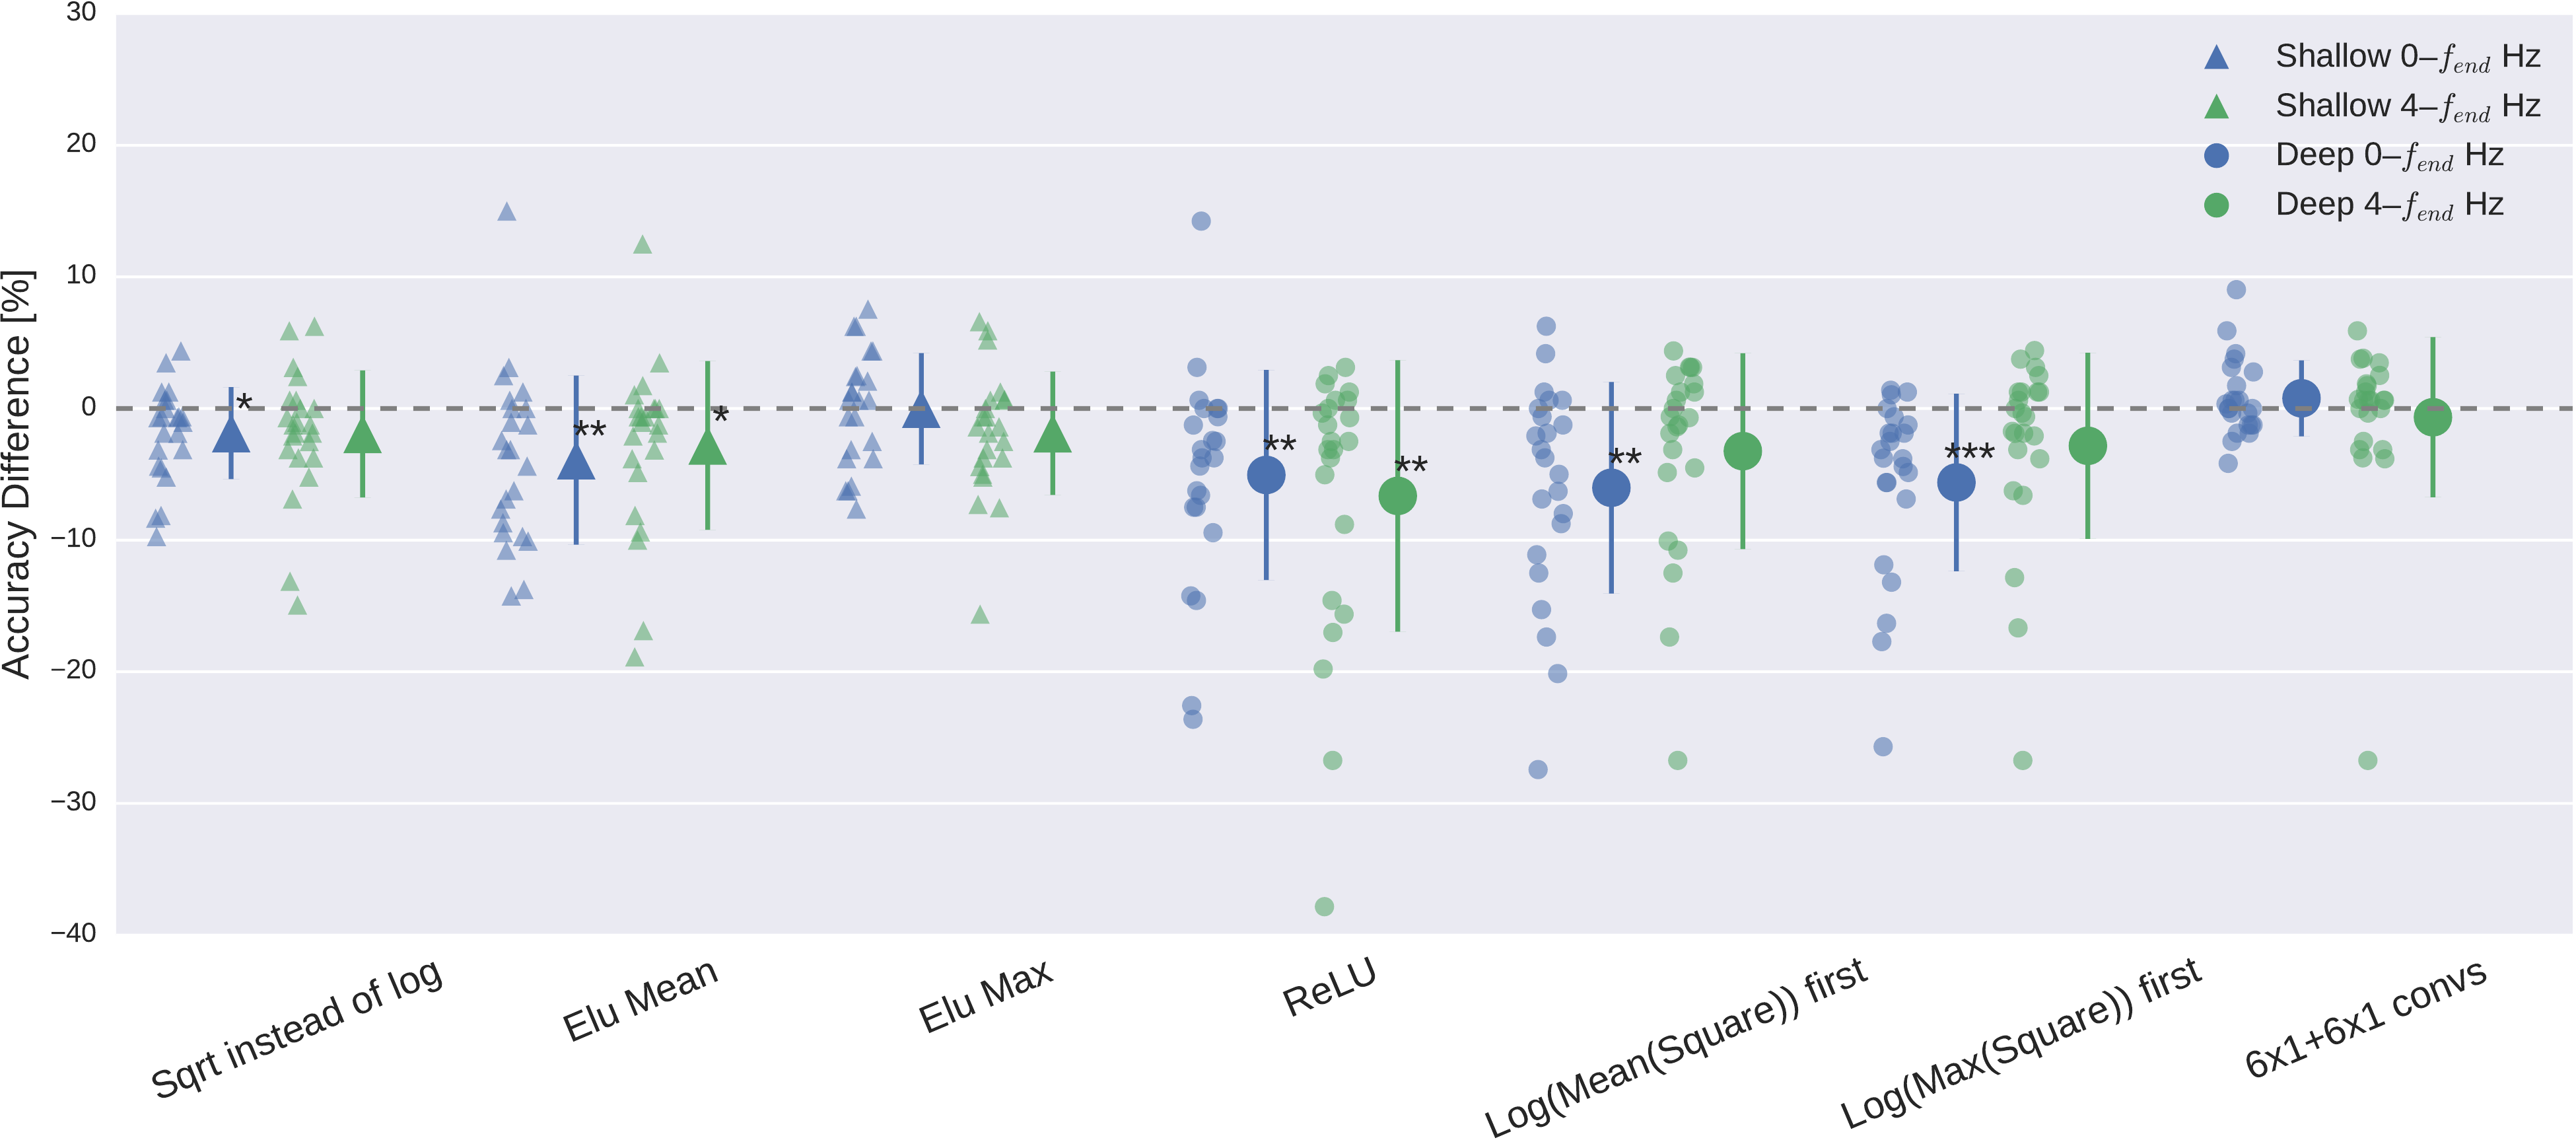
\includegraphics[width=0.9\linewidth]{images/Final_Comparison.ipynb.10.pdf-1.png}
    }
    \caption[Impact of ConvNet design choices on decoding accuracy]{
    \textbf{Impact of ConvNet design choices on decoding accuracy.} 
Accuracy differences of baseline and design choices on x-axis for the $0-f_\textrm{end}$ Hz and $4-f_\textrm{end}$ Hz datasets. 
Each small marker represents accuracy difference for one subject, and each larger marker represents mean accuracy difference across all subjects of both datasets. Bars: standard error of the differences across subjects. 
Stars indicate statistically significant differences to baseline (Wilcoxon signed-rank test, P < 0.05: $\diamond$\*, P < 0.01: $\diamond\diamond$\*\*, P < 0.001=\*\*\*). Top: Impact of design choices applicable to both ConvNets. 
All statistically significant differences were accuracy decreases from removing an aspect of our architecture.
Notably, there was a clear negative effect of removing both dropout and batch normalization. Bottom: Impact of different types of nonlinearities, pooling modes and filter sizes. Results are given independently for the deep ConvNet and the shallow ConvNet.
As before, all statistically significant differences were from accuracy decreases. Notably, replacing ELU by ReLU as nonlinearity led to decreases on both frequency ranges, which were both statistically significant. 
Figure from \citet{schirrmeisterdeephbm2017}.
}
\label{design-choices-fig}
\end{figure}

    Design choices substantially affected deep network accuracies on both
datasets, meaning BCI Competition IV 2a and the High Gamma Dataset.
Batch normalization and dropout significantly increased accuracies. This
became especially clear when omitting both simultaneously
\Cref{design-choices-fig}. Batch normalization provided a
larger accuracy increase for the shallow ConvNet, whereas dropout
provided a larger increase for the deep ConvNet. For both networks and
for both frequency bands, the only statistically significant accuracy
differences were accuracy decreases after removing dropout for the deep
ConvNet on $0-f\_\textrm{end}$ Hz data or removing batch
normalization and dropout for both networks and frequency ranges
($p<0.05$, Wilcoxon signed-rank test). Usage of tied loss did not
affect the accuracies very much, never yielding statistically
significant differences ($p>0.05$). Splitting the first layer into two
convolutions had the strongest accuracy increase on the
$0-f\_\textrm{end}$ Hz data for the shallow ConvNet, where it is also
the only statistically significant difference ($p<0.01$).

\section{Cropped Training Strategy Improved Deep ConvNet on Higher
Frequencies}\label{cropped-training-strategy-improved-deep-convnet-on-higher-frequencies}

\begin{figure}[htb]
    \myfloatalign
    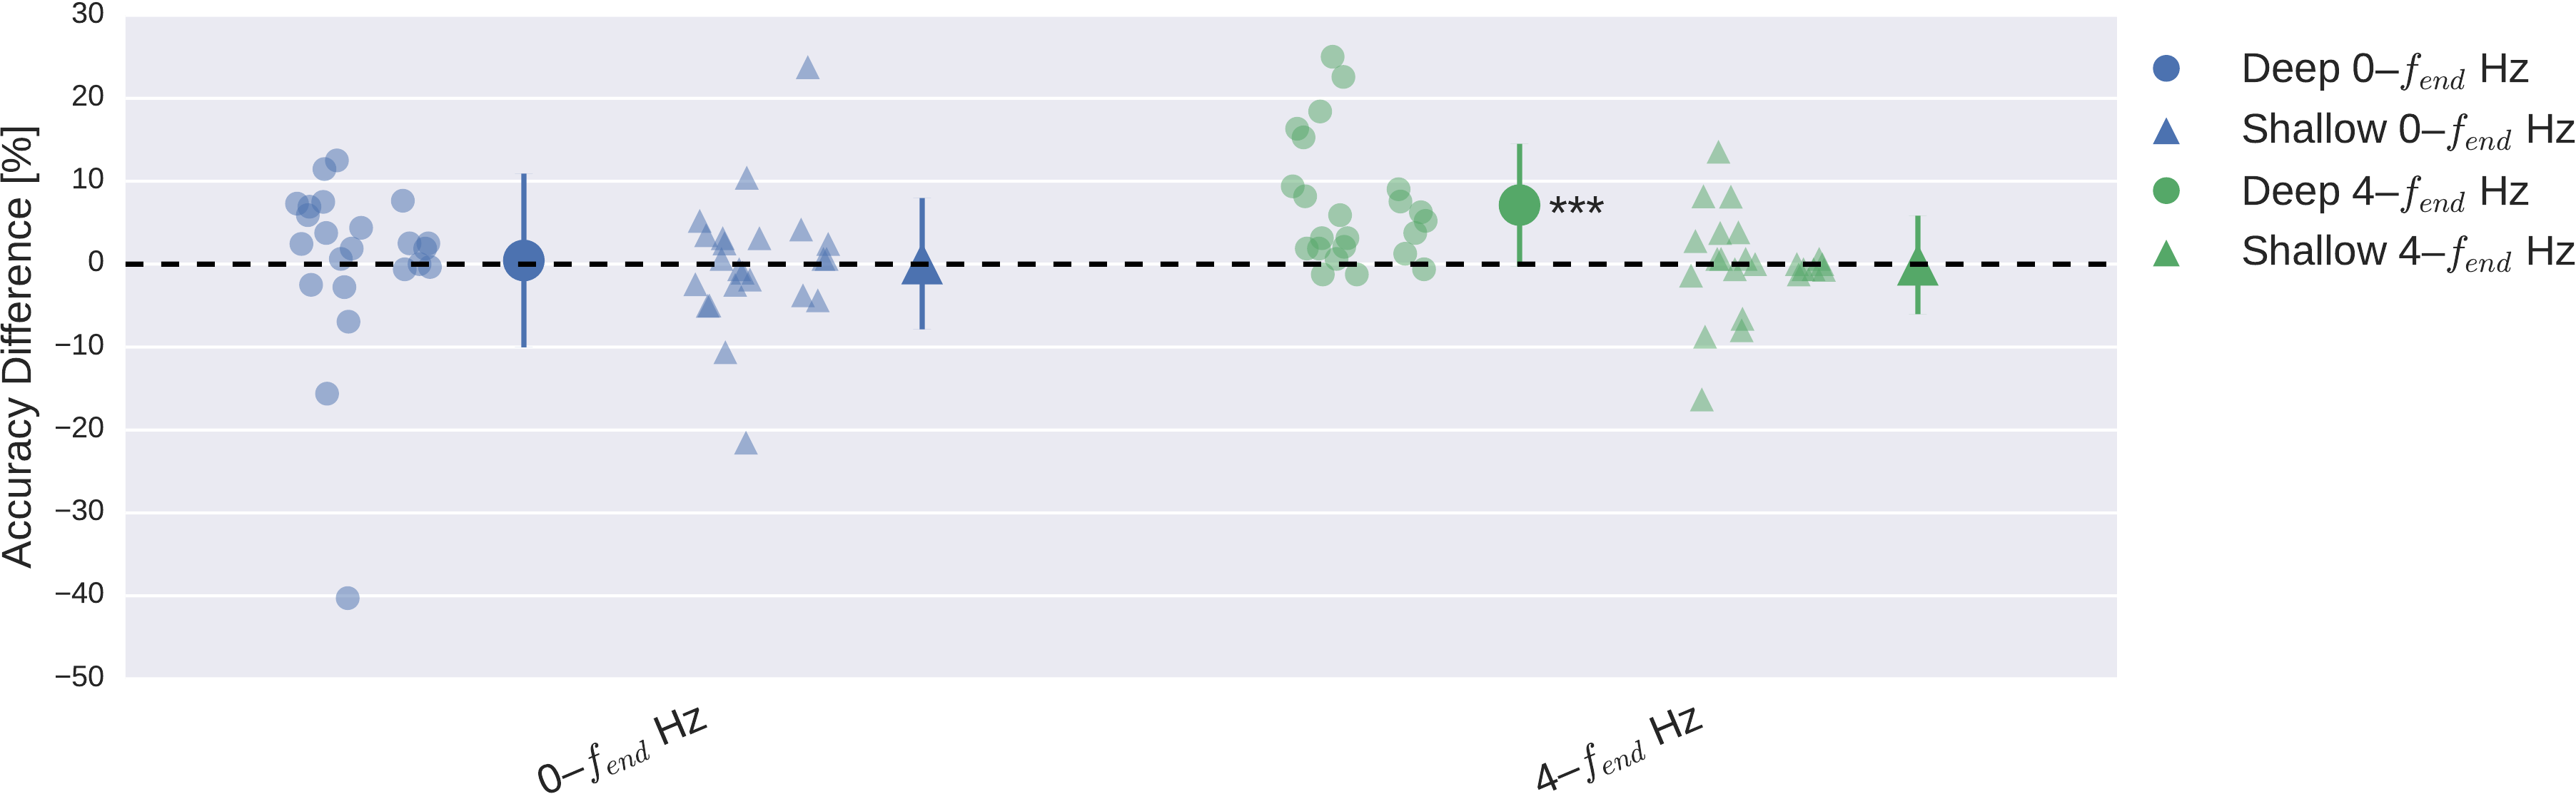
\includegraphics[width=1\linewidth]{images/Final_Comparison.ipynb.8.pdf-1.png}
    
    \caption[Impact of training strategy on decoding accuracy]{
\textbf{Impact of training strategy (cropped vs trial-wise training) on
accuracy.} Accuracy difference for both frequency ranges and both
ConvNets when using cropped training instead of trial-wise training.
Other conventions as in \Cref{design-choices-b-fig}. Cropped
training led to better accuracies for almost all subjects for the deep
ConvNet on the $4-f_\textrm{end}$-Hz frequency range. Figure from
\citet{schirrmeisterdeephbm2017}. 
}
\label{cropped-training-results-fig}
\end{figure}

    Cropped training increased accuracies statistically significantly for
the deep ConvNet on the $4-f_\textrm{end}$-Hz data (p\textless1e-5,
Wilcoxon signed-rank test, see
\Cref{cropped-training-results-fig}). In all other settings
($0-f_\textrm{end}$-Hz data, shallow ConvNet), the accuracy
differences were not statistically significant (p\textgreater0.1) and
showed a lot of variation between subjects.

\section{Results on BCI Competition IV
2b}\label{results-on-bci-competition-iv-2b}


\begin{table}[htb]
    \myfloatalign
    \begin{tabularx}{\textwidth}{lll}
    \toprule
        \tableheadlinewithwidth{0.2\textwidth}{FBCSP} & \tableheadlinewithwidth{0.2\textwidth}{Deep ConvNet} &
        \tableheadlinewithwidth{0.2\textwidth}{Shallow ConvNet} 
        \\
        \midrule
0.599 & -0.001 & +0.030 \\
        \bottomrule
    \end{tabularx}
    \caption[Kappa values on the BCIC IV 2b dataset]{
\textbf{Kappa values on the BCIC IV 2b dataset.} ConvNet
kappa values show the difference to the FBCSP kappa value.
    }  \label{bcic-iv-2b-results}
\end{table}


    To ensure that the results also generalize to further datasets and also
rule out hyperparameter overfitting, the FBCSP pipeline and the deep
network pipelines were applied with the exact same hyperparameters on
BCI Competition IV 2b. A few choices like the use of the decoding time
window had been done after already seeing results from the evaluation
sets of the High-Gamma dataset and the BCIC IV 2a dataset, hence it was
valuable to validate the results on the BCIC IV 2b dataset. Results in
\Cref{bcic-iv-2b-results} show that the networks perform as
good or better than FBCSP. Results on further datasets, also
non-movement-decoding datasets are presented in the next chapter
\Cref{task-related}.

\section{ConvNet-Independent
Visualizations}\label{convnet-independent-visualizations}



\begin{figure}[htb]
    \myfloatalign
    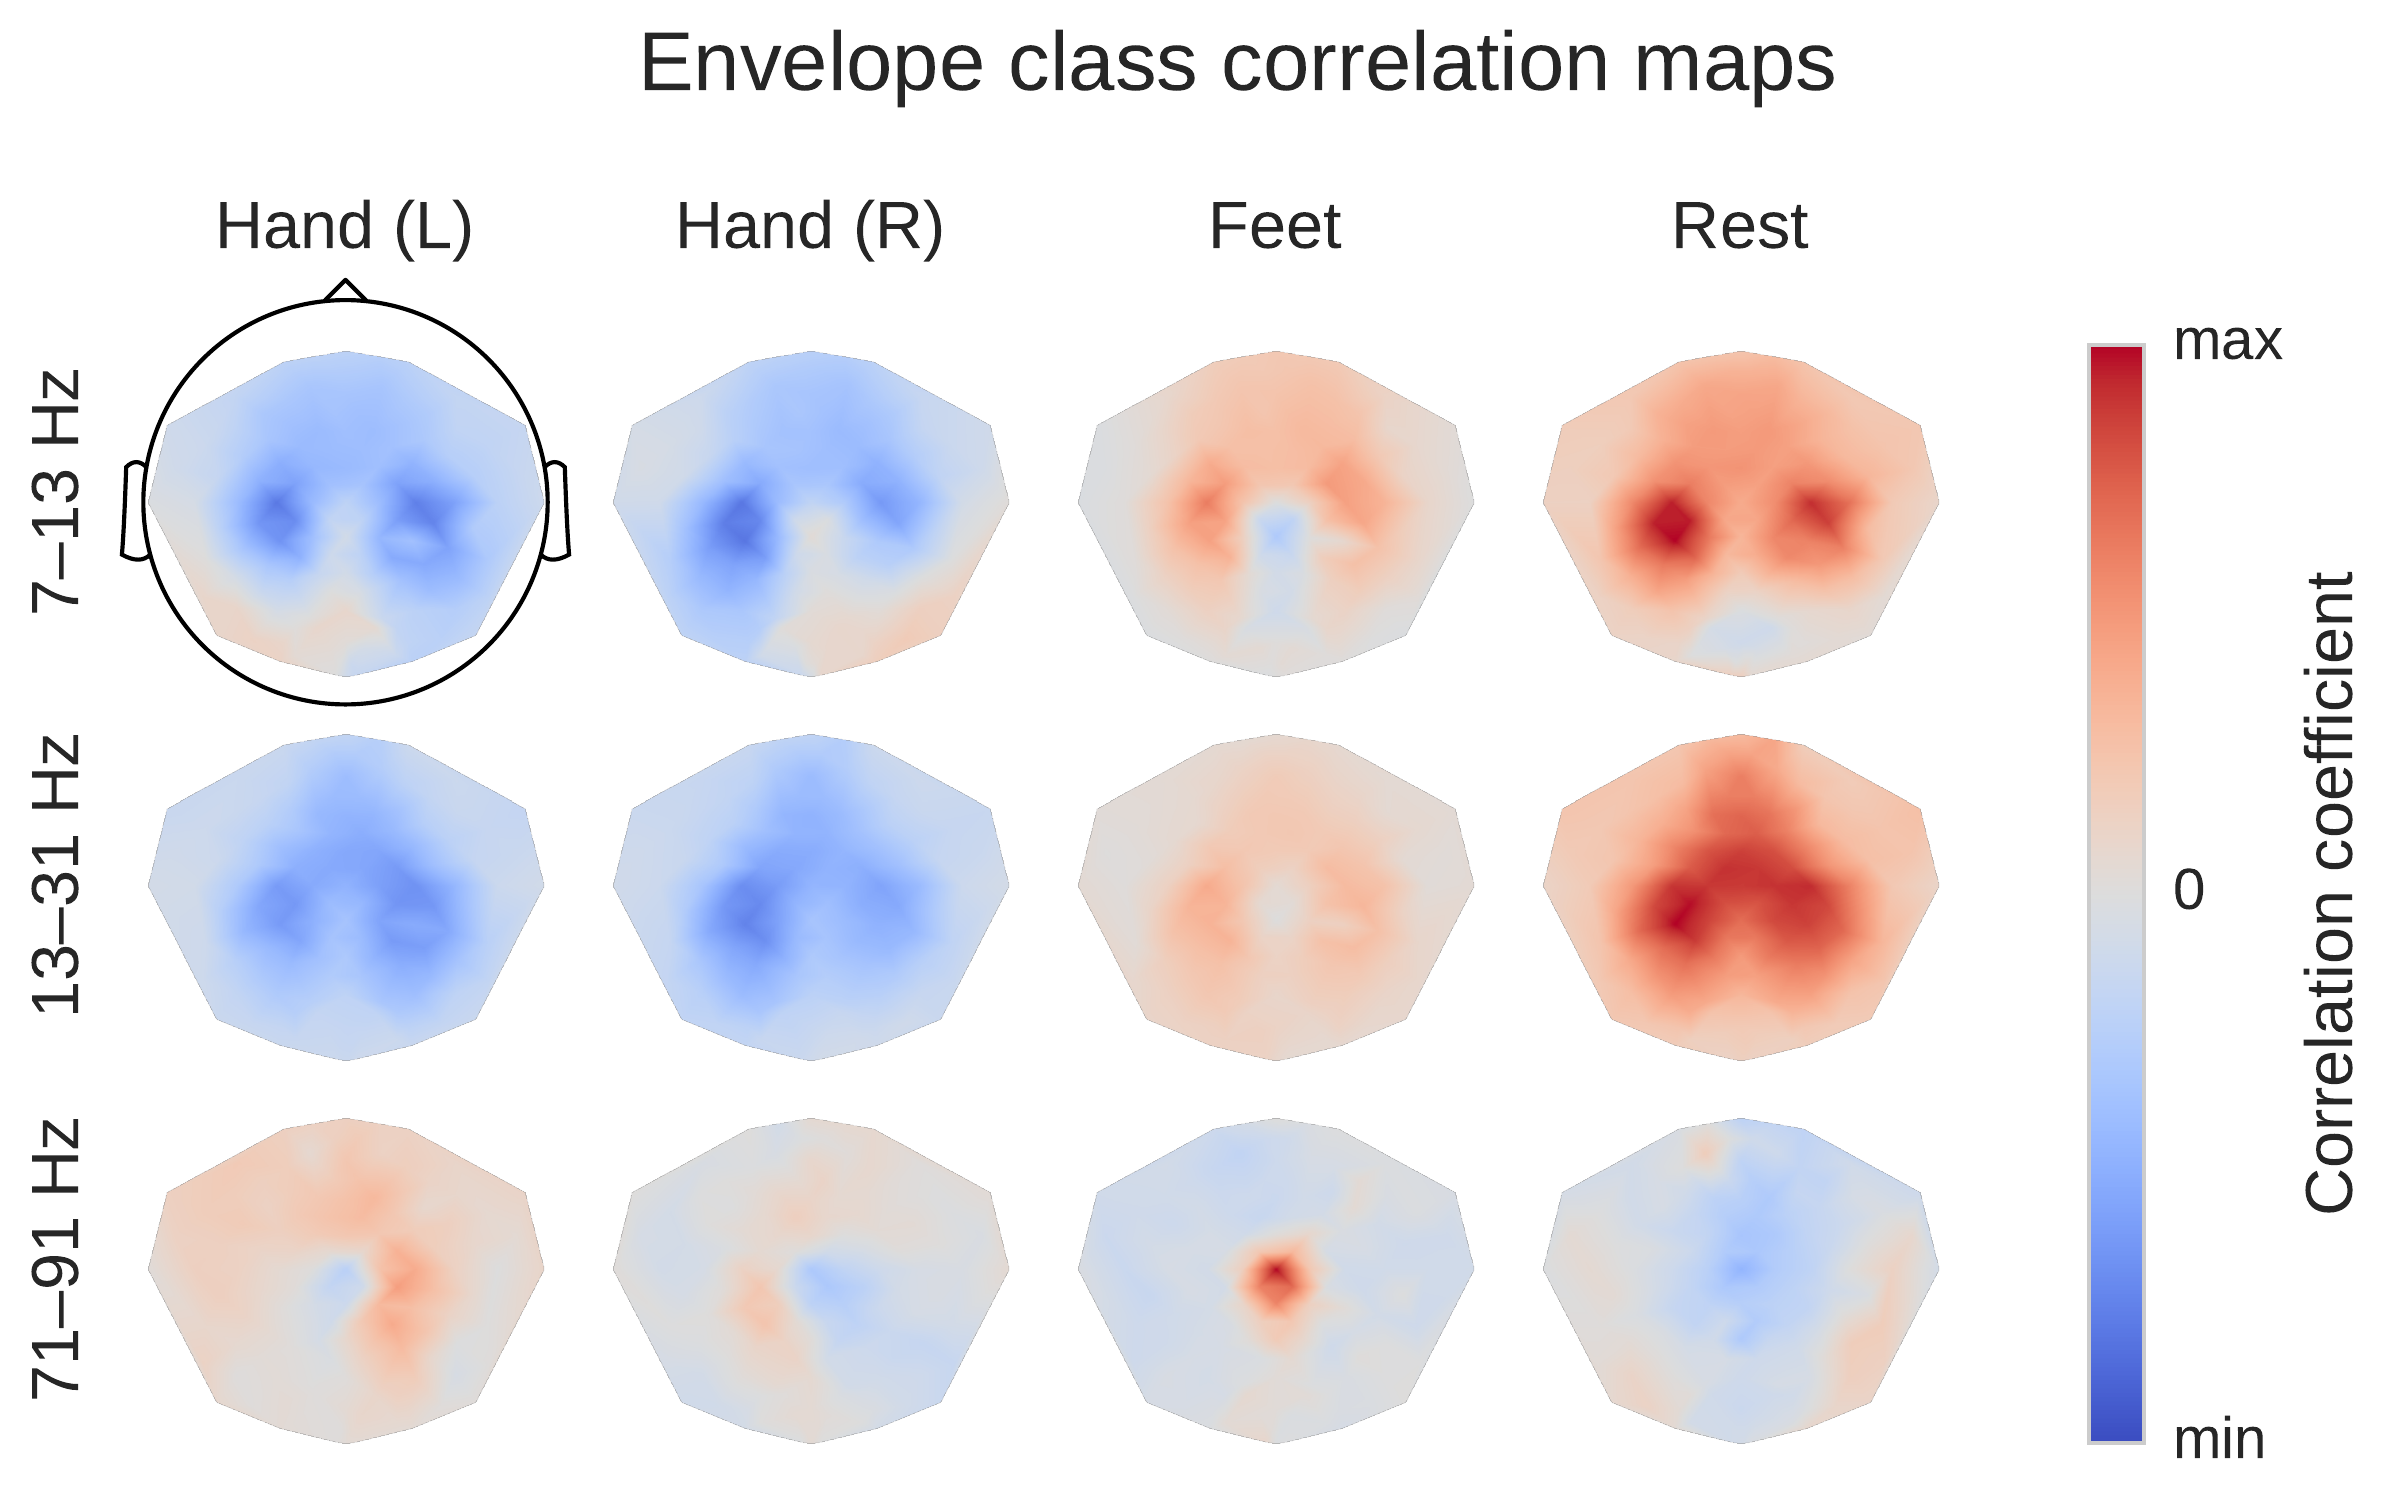
\includegraphics[width=1\linewidth]{images/Envelope_Correlations.ipynb.1.pdf-1.png}
    
    \caption[Envelope correlations on high-gamma dataset]{
\textbf{Average envelope correlations over subjects from the high-gamma dataset.} Colormaps are scaled per frequency band/row. This is a ConvNet-independent
visualization. Scalp plots show spatial distributions of class-related
spectral amplitude changes well in line with the literature. Figure from
\citet{schirrmeisterdeephbm2017}.
}
\label{envelope-class-fig}
\end{figure}


    Before moving to ConvNet visualization, we examined the spectral
amplitude changes associated with the different movement classes in the
alpha, beta and gamma frequency bands. For that, we first computed the
moving average of the squared envelope in narrow frequency bands via the
Hilbert transform as a measure of the power in those frequency bands.
Then we computed linear correlations of these moving averages with the
class label. This results in frequency-resolved envelope-class label
correlations.

We found the expected overall scalp topographies (see
\Cref{envelope-class-fig}) to show physiologically plausible
patterns. For example, for the alpha (7--13 Hz) frequency band, there
was a class-related power decrease (anti-correlation in the
class-envelope correlations) in the left and right pericentral regions
with respect to the hand classes, stronger contralaterally to the side
of the hand movement , i.e., the regions with pronounced power decreases
lie around the primary sensorimotor hand representation areas. For the
feet class, there was a power decrease located around the vertex, i.e.,
approx. above the primary motor foot area. As expected, opposite changes
(power increases) with a similar topography were visible for the gamma
band (71--91 Hz).

\section{Amplitude Perturbation
Visualizations}\label{amplitude-perturbation-visualizations}



\begin{figure}[t!hb]
    \myfloatalign
    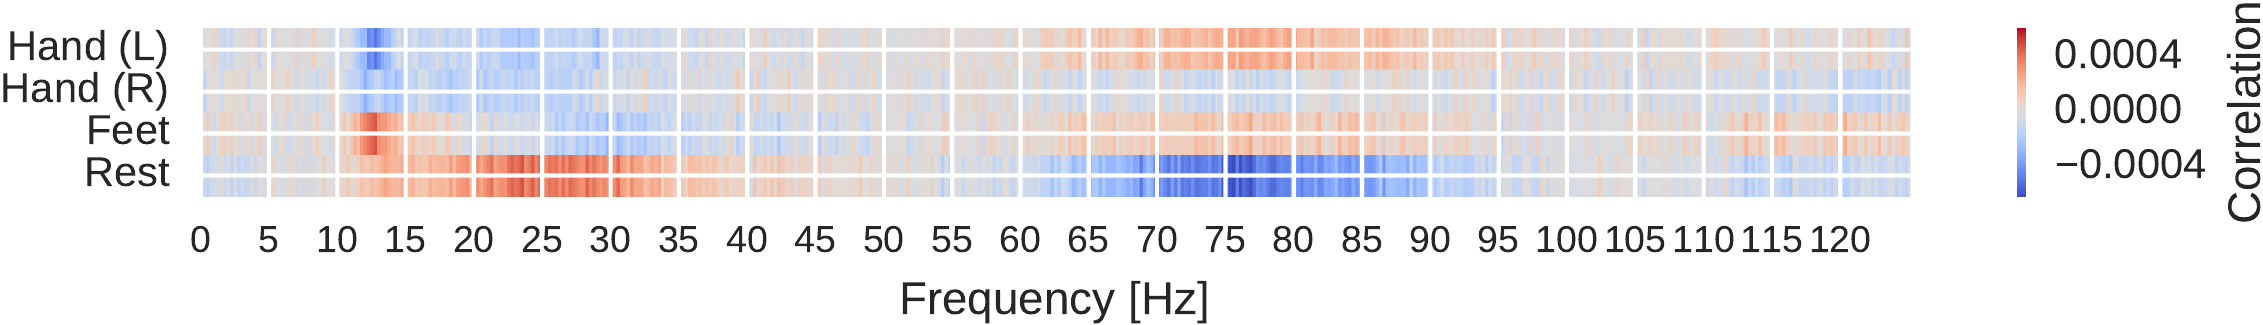
\includegraphics[width=1\linewidth]{images/Bandpower_Perturbation.ipynb.0.pdf-1.png}
    
    \caption[Per-class amplitude perturbation correlation profiles on high-gamma dataset]{
\textbf{Input-perturbation network-prediction correlations for all
frequencies for the deep ConvNet, per class.} Plausible correlations,
for example, rest positively, other classes negatively correlated with
the amplitude changes in frequency range from 20 to 30 Hz. Figure from
\citet{schirrmeisterdeephbm2017}.
}
\label{bandpower-perturbation-per-class-fig}
\end{figure}


\begin{figure}[htb]
    \myfloatalign
    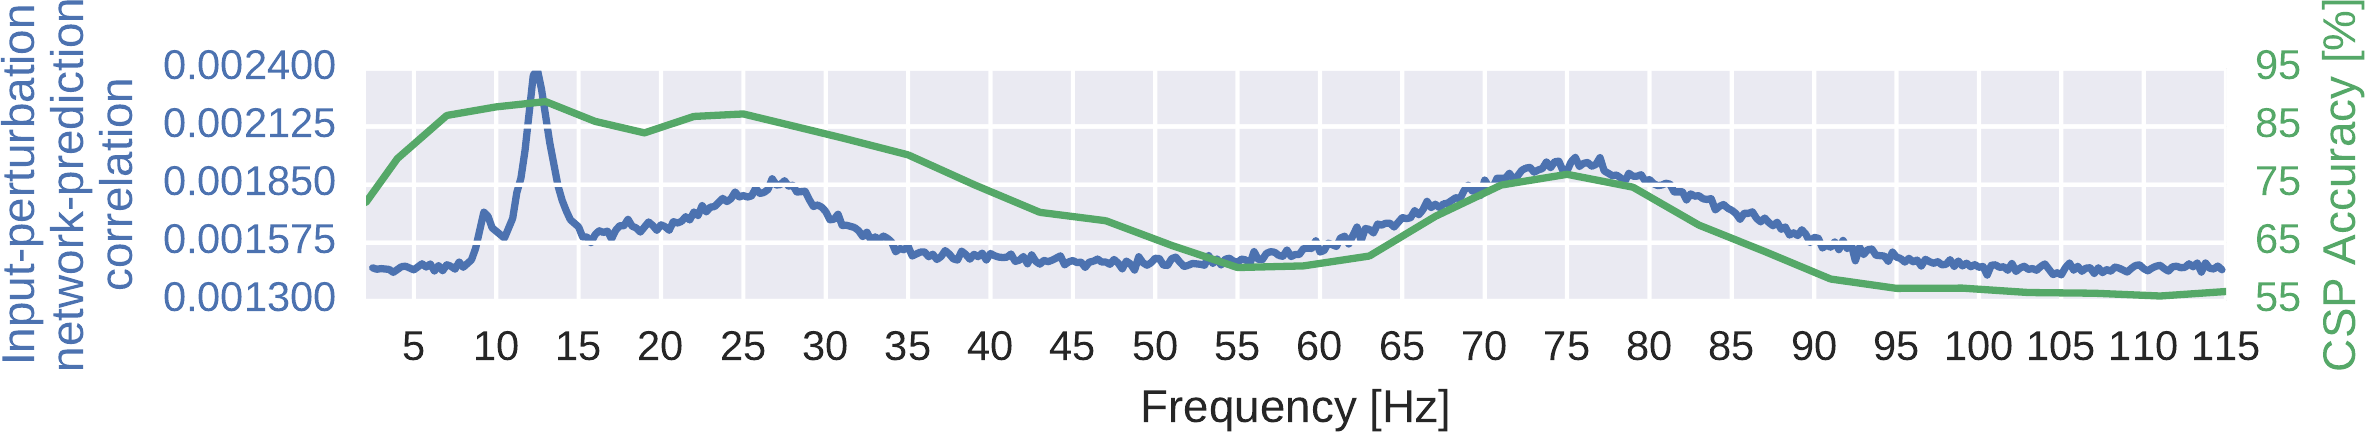
\includegraphics[width=1\linewidth]{images/Bandpower_Perturbation.ipynb.12.pdf-1.png}
    
    \caption[Overall amplitude perturbation correlation profile on high-gamma dataset]{
\textbf{Absolute input-perturbation network-prediction correlation
frequency profile for the deep ConvNet.} Mean absolute correlation value
across classes. CSP binary decoding accuracies for different frequency
bands for comparison, averaged across subjects and class pairs. Peaks in
alpha, beta, and gamma band for input-perturbation network-prediction
correlations and CSP accuracies. Figure from
\citet{schirrmeisterdeephbm2017}.
}
\label{bandpower-overall-fig}
\end{figure}

Our amplitude perturbation visualizations show that the network have
learned to extract commonly used spectral amplitude features.We show
three visualizations extracted from input-perturbation
network-prediction correlations, the first two to show the frequency
profile of the causal effects, the third to show their topography. Thus,
first, we computed the mean across electrodes for each class separately
to show correlations between classes and frequency bands. We see
plausible results, for example, for the rest class, positive
correlations in the alpha and beta bands and negative correlations in
the gamma band in
\Cref{bandpower-perturbation-per-class-fig}.



    Then, second, by taking the mean of the absolute values both over all
classes and electrodes, we computed a general frequency profile. This
showed clear peaks in the alpha, beta, and gamma bands
(\Cref{bandpower-overall-fig}). Similar peaks were seen in
the means of the CSP binary decoding accuracies for the same frequency
range.


\begin{figure}[htb]
    \myfloatalign
    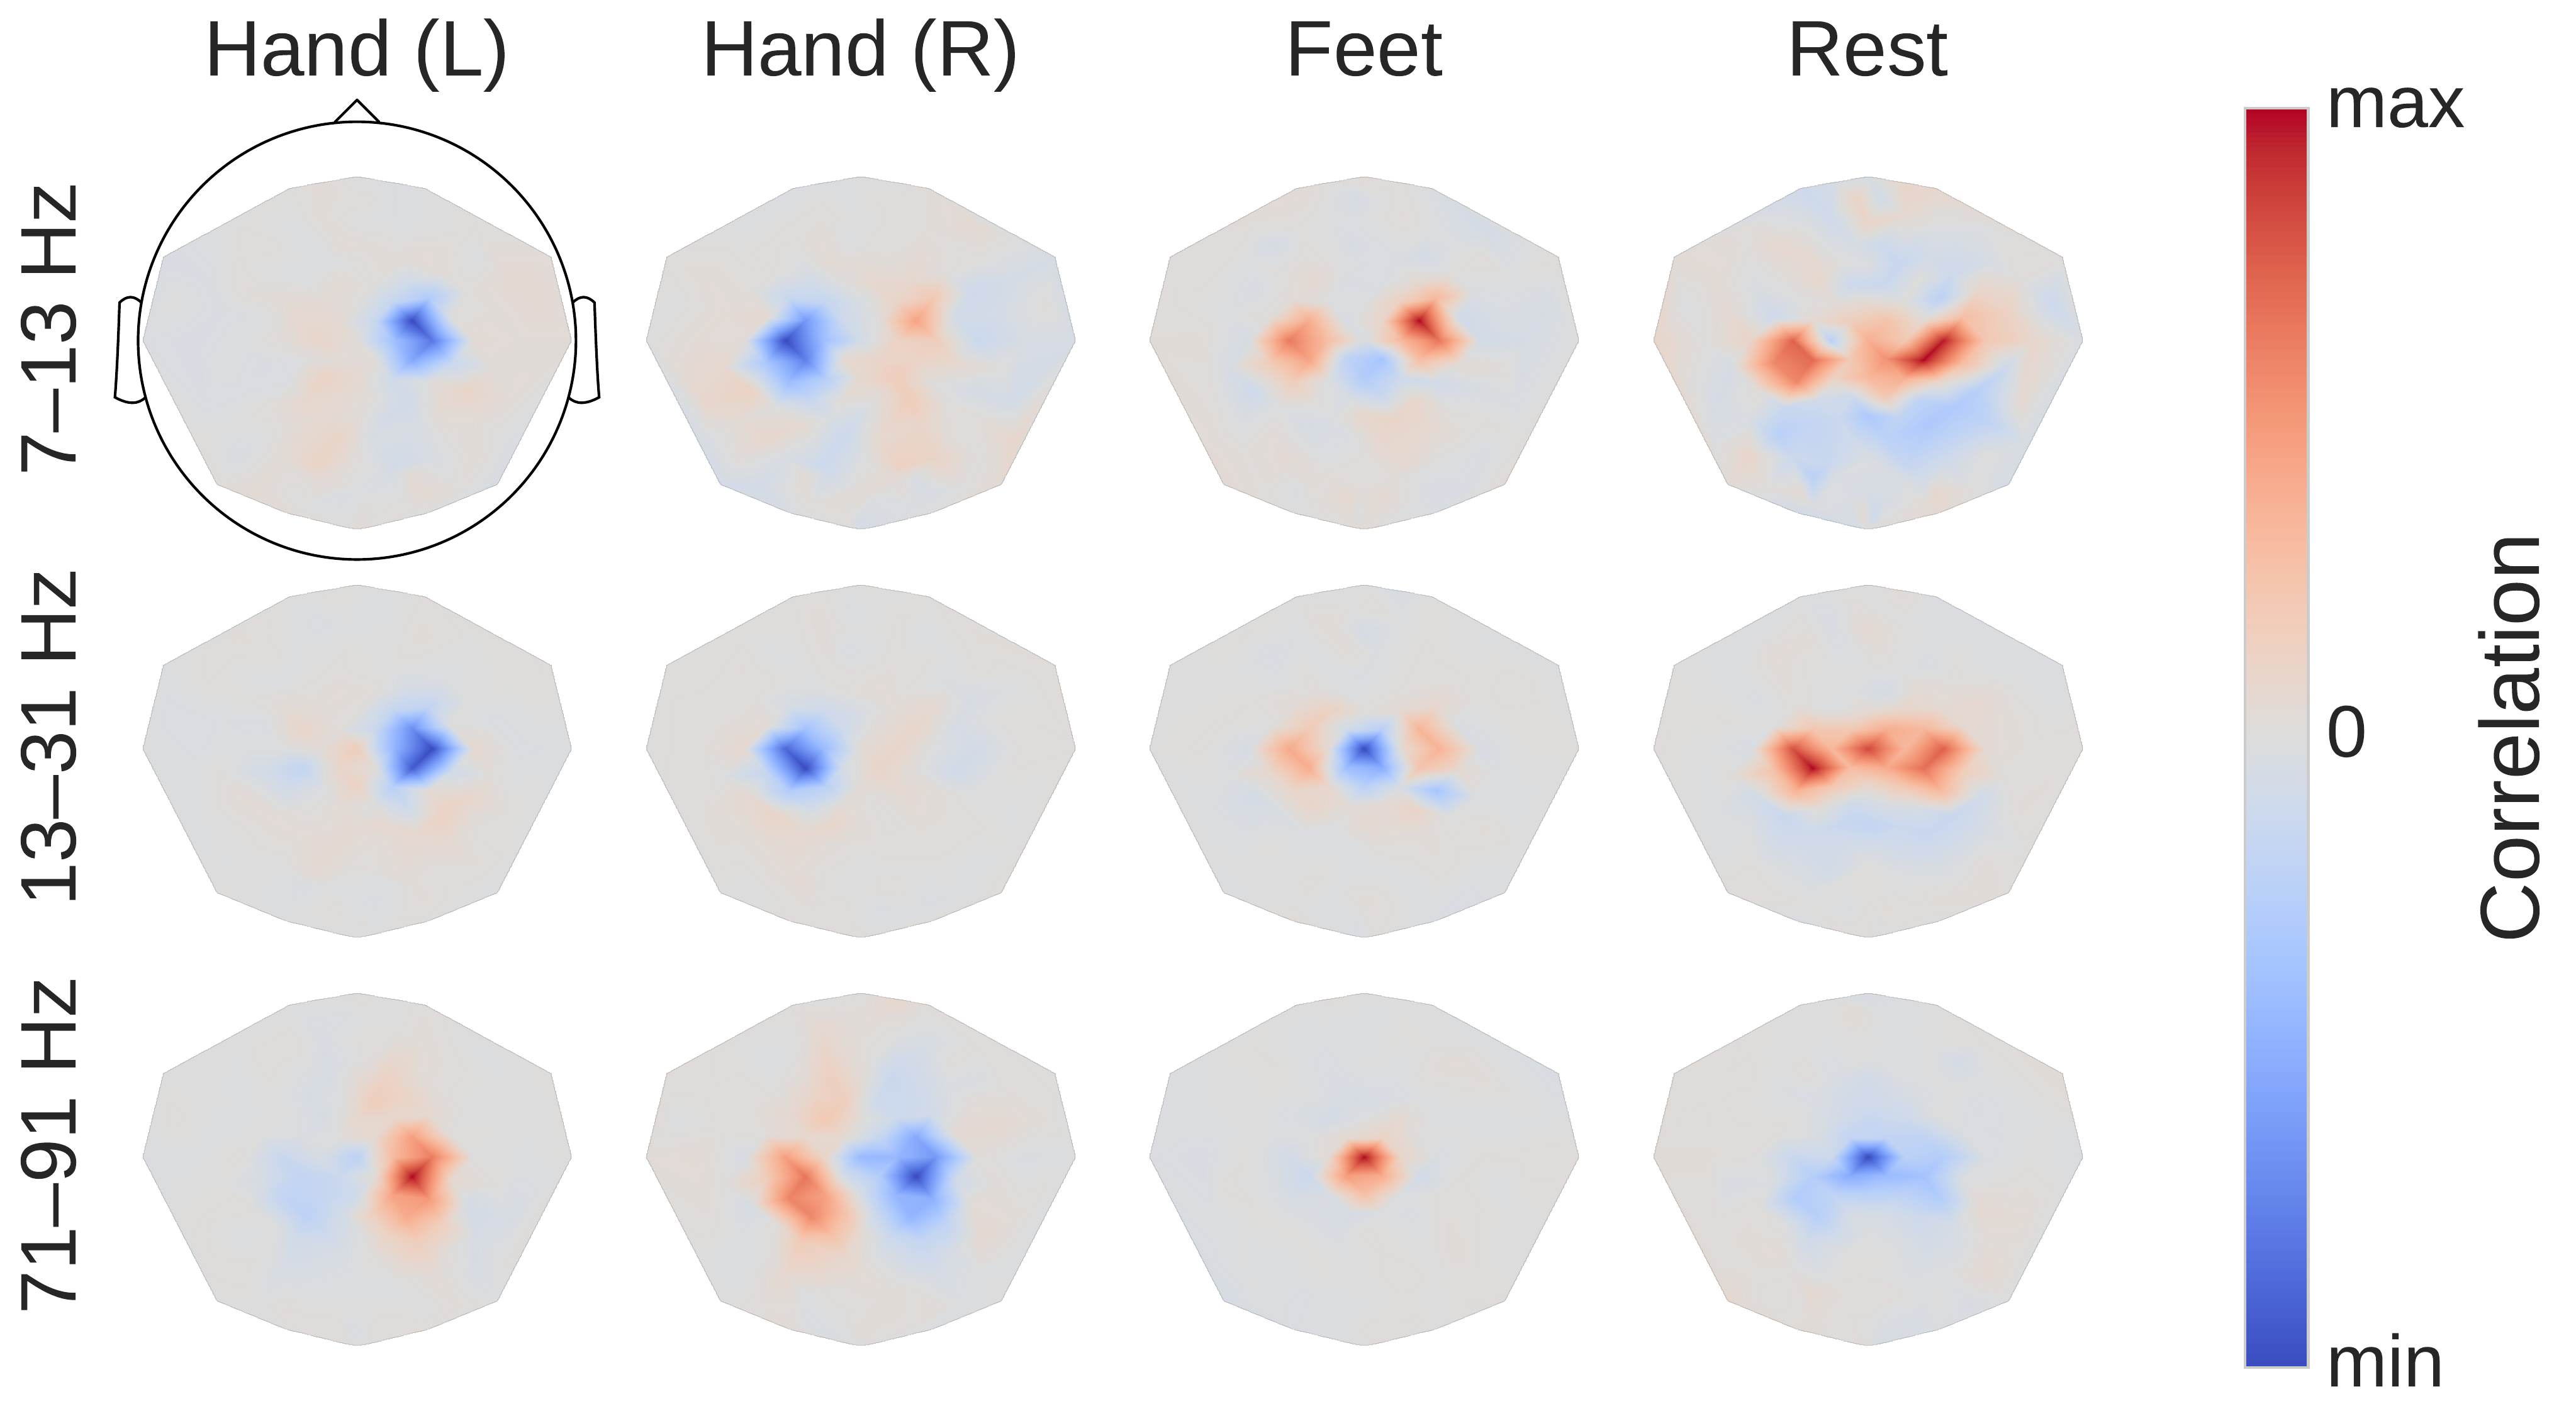
\includegraphics[width=1\linewidth]{images/Bandpower_Perturbation.ipynb.3.pdf-1.png}
    
    \caption[Amplitude perturbation correlation scalp plots on high-gamma dataset]{
\textbf{Input-perturbation network-prediction correlation maps for the
deep ConvNet.} Correlation of class predictions and amplitude changes.
Averaged over all subjects of the High-Gamma Dataset. Colormaps are
scaled per scalp plot. Plausible scalp maps for all frequency bands, for
example, contralateral positive correlations for the hand classes in the
gamma band. Figure from \citet{schirrmeisterdeephbm2017}.
}
\label{bandpower-perturbation-topo-fig}
\end{figure}




    Third, scalp maps of the input-perturbation effects on network
predictions for the different frequency bands, as shown in
\Cref{bandpower-perturbation-topo-fig}, show spatial
distributions expected for motor tasks in the alpha, beta and --- for
the first time for such a noninvasive EEG decoding visualization --- for
the high gamma band. These scalp maps directly reflect the behavior of
the ConvNets and one needs to be careful when making inferences about
the data from them. For example, the positive correlation on the right
side of the scalp for the Hand (R) class in the alpha band only means
the ConvNet increased its prediction when the amplitude at these
electrodes was increased independently of other frequency bands and
electrodes. It does not imply that there was an increase of amplitude
for the right hand class in the data. Rather, this correlation could be
explained by the ConvNet reducing common noise between both locations,
for more explanations of these effects in case of linear models, see
\Cref{perturbation-visualization-interpretation} and
\cite{haufe_interpretation_2014}. Nevertheless, for the
first time in noninvasive EEG, these maps clearly revealed the global
somatotopic organization of causal contributions of motor cortical gamma
band activity to decoding right and left hand and foot movements.
Interestingly, these maps revealed highly focalized patterns,
particularly during hand movement in the gamma frequency range
(\Cref{bandpower-perturbation-topo-fig}, first plots in last
row), in contrast to the more diffuse patterns in the conventional
task-related spectral analysis as shown in
\Cref{envelope-class-fig}.

\section{Internal Representations of Amplitude and
Phase}\label{internal-representations-of-amplitude-and-phase}

\begin{figure}[htb]
    \myfloatalign
    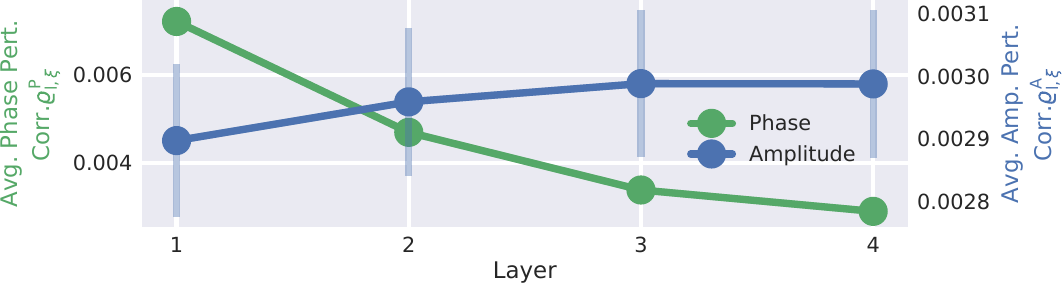
\includegraphics[width=1\linewidth]{images/PhaseAmpDev_.pdf-1.png}
    
    \caption[Mean phase and amplitude perturbation correlations over layers]{
\textbf{Mean phase and amplitude perturbation correlations over layers.}
Curves show mean perturbation correlation over all frequencies for each
layer. Scales are different and written on the left and right y-axes.
The error bars show the standard error over the subjects. Standard
errors for phase and amplitude are similar, but much higher relatively
in the amplitude correlation scale and therefore only visible there. In
their respective scale, curves show a clearly inverse behavior over the
layers with increasing amplitude correlations and decreasing phase
correlations. Figure from \citet{hartmann2018hierarchical} (© 2018 IEEE).
}
\label{phase-amp-dev-layer-fig}
\end{figure}


\begin{figure}[htb]
    \myfloatalign
    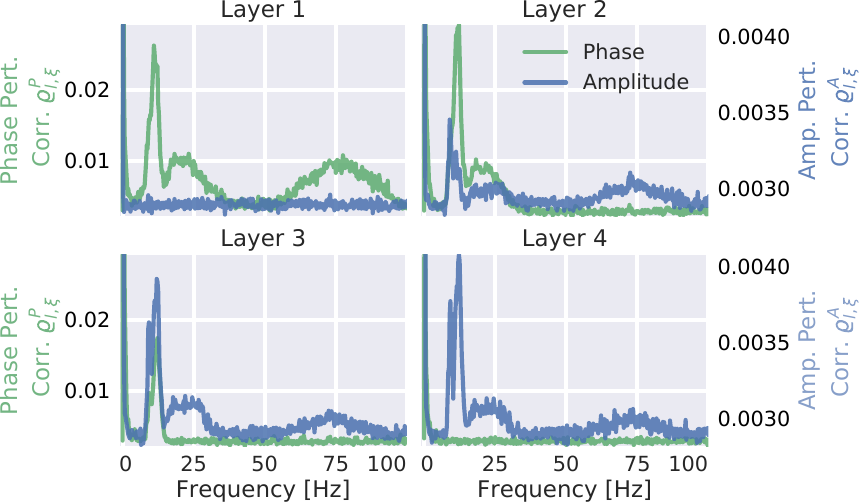
\includegraphics[width=1\linewidth]{images/PhaseAmp.pdf-1.png}
    
    \caption[Mean of absolute phase and amplitude perturbation correlations
for individual frequencies]{
\textbf{Mean of absolute phase and amplitude perturbation correlations
for individual frequencies.} The two correlation types have different
scales, denoted by the left and right y-axis. As in
\Cref{phase-amp-dev-layer-fig}, a clearly inverse relation
between amplitude and phase correlations is visible. This visualization
additionally showed that alpha (7-13 Hz), beta (13-30 Hz), and high
gamma (50-100 Hz) frequency ranges each have a specific layer in which
their phase correlation vanishes and their amplitude correlation
saturates (high gamma in layer 2, beta in layer 3, and alpha in layer
4). Figure from \citet{hartmann2018hierarchical} (© 2018 IEEE).
}
\label{phase-amp-layer-fig}
\end{figure}


    The perturbation analysis showed that the earlier layers represent more
phase-specific features than later layers, while the later layers
represent more phase-invariant amplitude features than the early layers.
\Cref{phase-amp-dev-layer-fig} shows the average absolute
phase perturbation correlation and amplitude perturbation correlation
over the 4 convolutional layers. The figure shows a clearly opposing
development of their respective average values across layers, with
increasing amplitude perturbation correlations and decreasing phase
perturbation correlations.

The perturbation correlations for individual frequencies showed a strong
phase perturbation correlation in the earlier layers 1 and 2 to phases
in the alpha, beta, and high gamma range (see
\Cref{phase-amp-layer-fig} ). The overall phase perturbation
correlation was highest in layer 1 and gradually became lower over
layers 2, 3, and 4. Interestingly, for each frequency band (alpha, beta,
and high gamma), there was one specific layer in which the phase
perturbation correlations vanished completely. Phase perturbation
correlations for high gamma vanished in layer 2, correlations for beta
vanished in layer 3, and correlations for alpha vanished in layer 4.
This vanishing of phase correlations for high gamma in layer 2 could be
observed in all subjects. For 4 subjects, alpha did already vanish
together with beta in layer 3.

An opposite behavior could be observed for amplitude correlations.
Notable phase insensitive amplitude perturbation correlations are only
emerging in layer 2. Amplitude correlations of individual frequency
bands peaked and saturated in the same layers in which the phase
correlation vanished: High gamma amplitude perturbation correlation
saturated in layer 2, beta in layer 3, and alpha in layer 4.

A potential underlying reason may be the use of max pooling with stride
3 after layers 1,2 and 3. The resulting temporal frequency resolutions
of the intermediate representations when only taking into account the
pooling strides are $\frac{250 \textrm{Hz}}{3} \approx 83\textrm{Hz}$,
$\frac{250 \textrm{Hz}}{3^2} \approx 28\textrm{Hz}$ and
$\frac{250 \textrm{Hz}}{3^3} \approx 9\textrm{Hz}$. The corresponding
Nyquist frequencies of approximately $41.5\textrm{Hz}$,
$14\textrm{Hz}$ and $4.5\textrm{Hz}$ seem to correspond to frequency
cutoffs above which the network is no longer phase-sensitive. However,
note that the network is in principle capable of retaining phase
sensitivity even in the presence of max pooling by shifting temporal
information to its channel dimension.

\section{Maximally Activating
Units}\label{maximally-activating-units}



\begin{figure}[h!tb]
    \captionsetup[subfigure]{labelformat=empty}
    \myfloatalign
    \subfloat[]
    {
    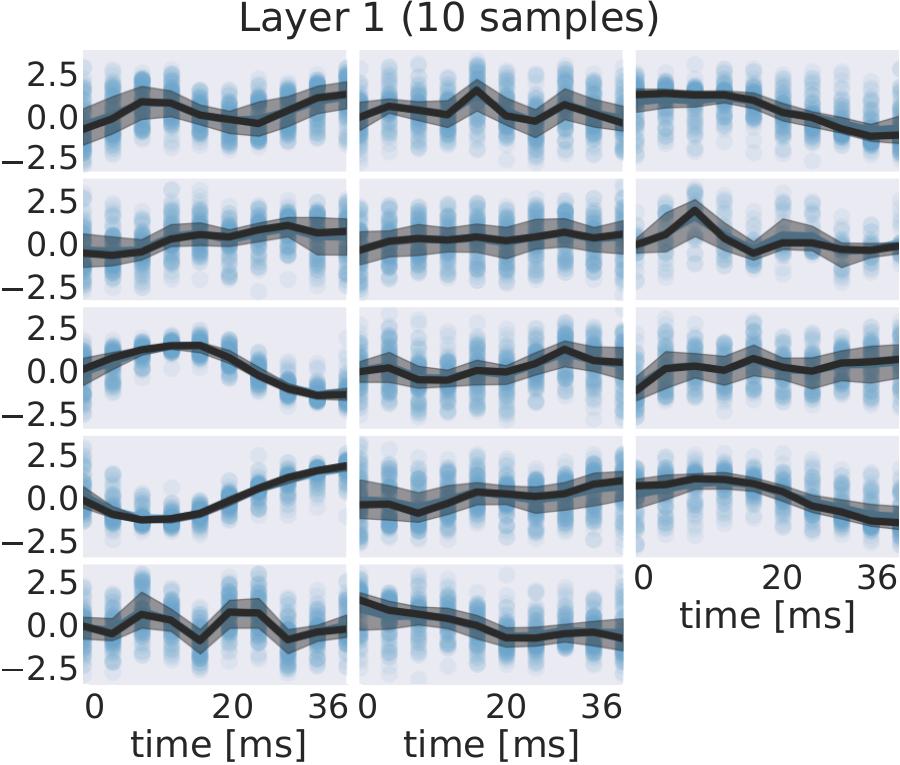
\includegraphics[width=.45\linewidth]{images/Inputs1_struct.pdf-1.png}} \quad
    \subfloat[] 
    {\
        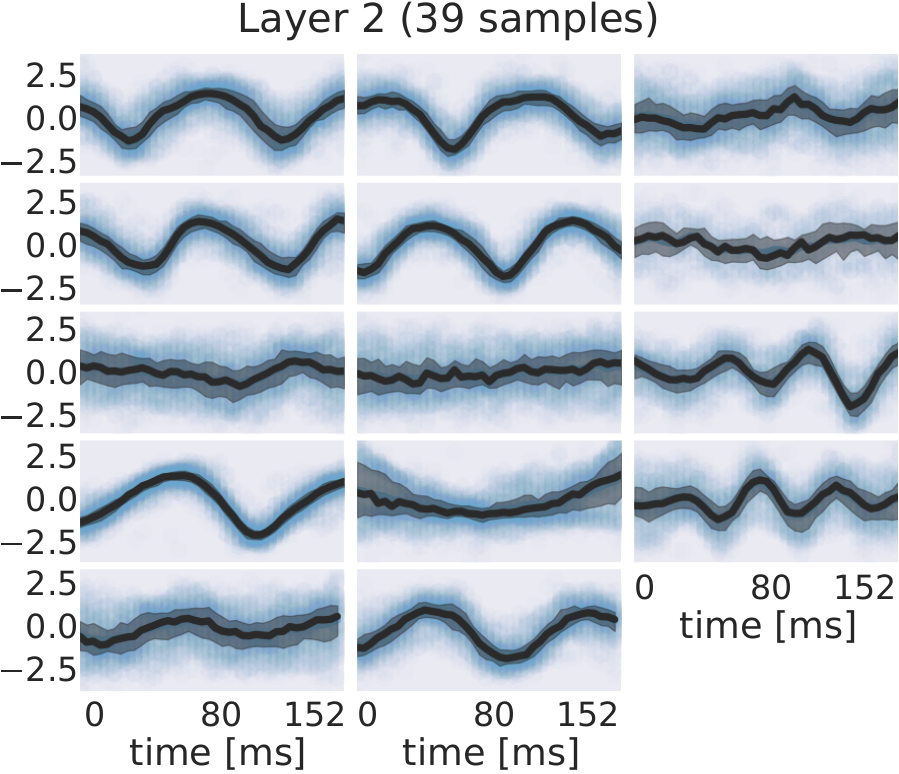
\includegraphics[width=.45\linewidth]{images/Inputs2_struct.pdf-1.png}} \\
    \subfloat[]
    {
    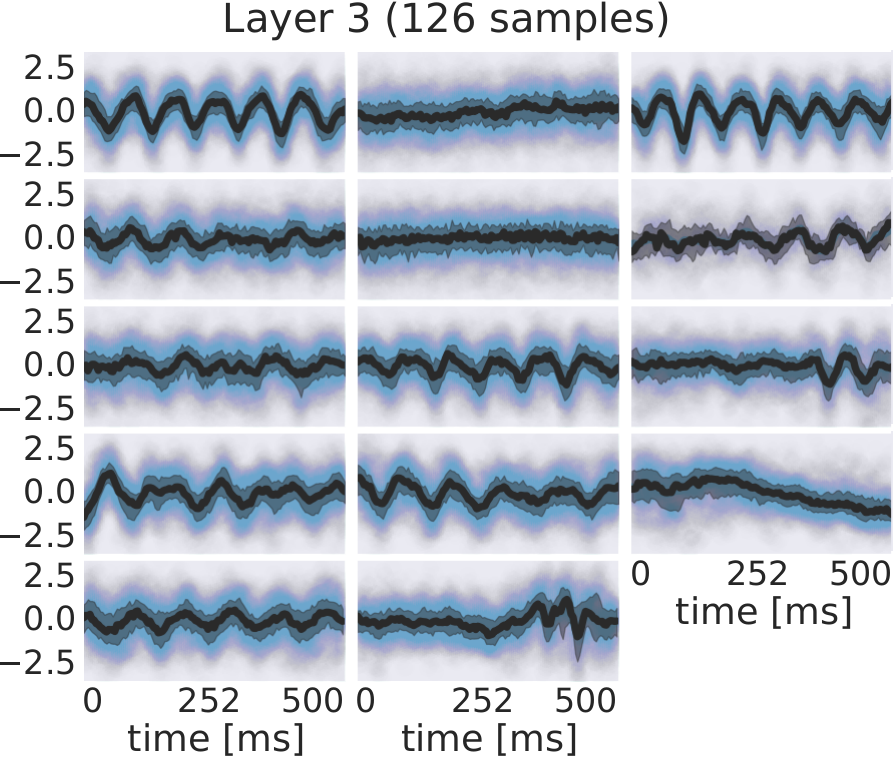
\includegraphics[width=.45\linewidth]{images/Inputs3_struct.pdf-1.png}} \quad
    \subfloat[]
    {
        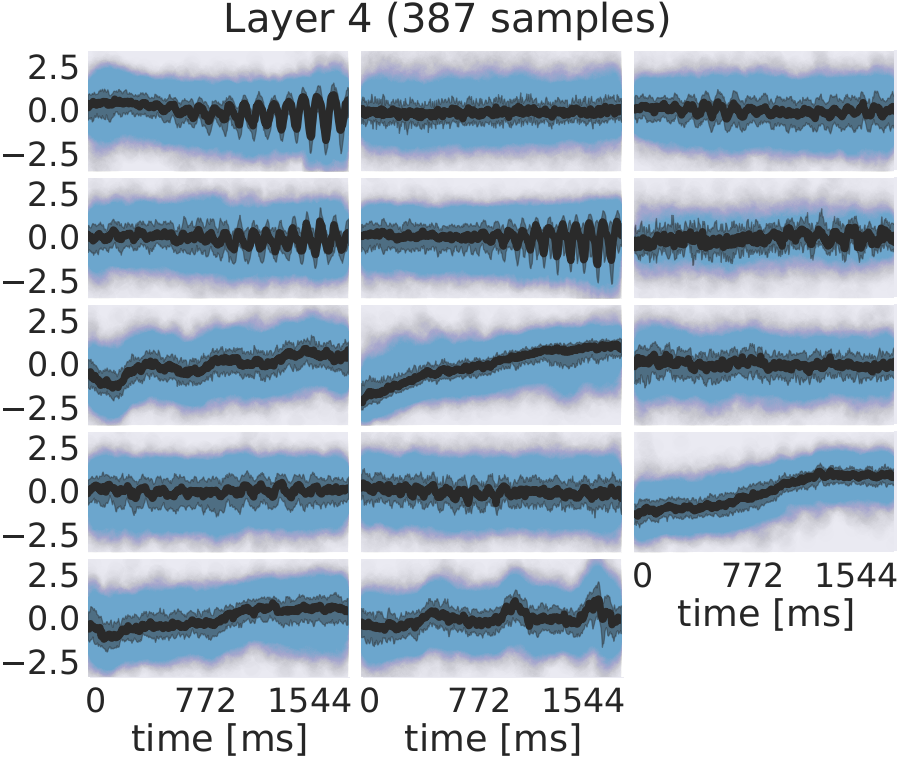
\includegraphics[width=.45\linewidth]{images/Inputs4_struct.pdf-1.png}} \\
    \caption[EEG signals in most-activating windows. per-electrode class prototypes]{
\textbf{EEG signals in most-activating input windows.} Taken from one randomly sampled filter in each layer for each subject. Blue points are the standard scores of all most-activating input windows for a filter. Their median is shown in black and the interquartile range as a gray shaded area. Medians in earlier layers often resemble parts of or complete sinusoids while medians in later layers resemble more complex
patterns. Figure from \citet{hartmann2018hierarchical} (© 2018 IEEE). 
    }\label{maximally-activating-units-fig}
\end{figure}



    In addition to examining how the individual layers respond to
frequency-specific phase and amplitude, we were also interested in other
characteristic features that might be learned by filters. To investigate
other features than frequency-specific phase or amplitude of sinusoidal
signals, we visually inspected the most-activating input windows of a
filter and their median values for each timepoint.
\Cref{maximally-activating-units-fig} shows the
most-activating input windows of one randomly sampled filter for each
subject and layer. We show each such set of most activating input
windows here at a representative electrode.
% 
For several filters, a clearly defined structure was present in the
median. The median plots for layer 1 show several examples of sinusoidal
shapes in different frequencies. Medians of higher frequencies were
sharper and the variance across input windows is larger. Medians of
layer 2 revealed several smooth alpha sinusoids, but also examples of
beta waves. In addition to that, there were some flat medians without an
easily interpretable periodicity or other temporal structure. In layer
3, there were mostly examples for alpha waves. For some medians in layer
4, more complex temporal patterns emerged. Those medians were relatively
flat at the beginning of the input windows, but showed an oscillatory
pattern with increasing amplitude in the later parts of the input
windows. Also, the oscillatory patterns in some examples resembled mu
waves more closely than pure sinusoids. Such patterns were found in
several subjects.

\section{Braindecode}\label{braindecode}

Work performed for this study also later led to the creation of the
open-source EEG deep learning library Braindecode, now with
contributions from multiple research groups and available at
\url{https://github.com/braindecode/braindecode/}.

\begin{openbox}
\item How well do ConvNets perform on other decoding tasks?
\item Do they work on tasks where oscillatory features are less important?
\item Do they work on non-trial based tasks like decoding pathology?
\end{openbox}
